% mnras_guide.tex
%
% MNRAS LaTeX user guide
%
% v3.1 released 11 June 2020
%
% v3.0 released 22 May 2015
% (version numbers match those of mnras.cls)
%
% Copyright (C) Royal Astronomical Society 2015
% Authors:
% Keith T. Smith (Royal Astronomical Society)

% Change log
%
% v3.0   September 2013 - May 2015
%    First version: complete rewrite of the user guide
%    Basic structure taken from mnras_template.tex by the same author

%%%%%%%%%%%%%%%%%%%%%%%%%%%%%%%%%%%%%%%%%%%%%%%%%%
% Basic setup. Most papers should leave these options alone.
\documentclass[fleqn,usenatbib,useAMS]{mnras}

%%%%% AUTHORS - PLACE YOUR OWN PACKAGES HERE %%%%%

% Only include extra packages if you really need them. Common packages are:
\usepackage{graphicx}	% Including figure files
\usepackage{amsmath}	% Advanced maths commands
\usepackage{amssymb}	% Extra maths symbols
\usepackage{multicol}        % Multi-column entries in tables
\usepackage{bm}		% Bold maths symbols, including upright Greek
\usepackage{pdflscape}	% Landscape pages

%%%%%%%%%%%%%%%%%%%%%%%%%%%%%%%%%%%%%%%%%%%%%%%%%%

%%%%%% AUTHORS - PLACE YOUR OWN MACROS HERE %%%%%%
\usepackage{subcaption}
% Please keep new commands to a minimum, and use \newcommand not \def to avoid
% overwriting existing commands. Example:
%\newcommand{\pcm}{\,cm$^{-2}$}	% per cm-squared
\newcommand{\kms}{\,km\,s$^{-1}$} % kilometres per second
\newcommand{\bibtex}{\textsc{Bib}\!\TeX} % bibtex. Not quite the correct typesetting, but close enough

%%%%%%%%%%%%%%%%%%%%%%%%%%%%%%%%%%%%%%%%%%%%%%%%%%


% Use vector fonts, so it zooms properly in on-screen viewing software
% Don't change these lines unless you know what you are doing
\usepackage[T1]{fontenc}
\usepackage{ae,aecompl}

% MNRAS is set in Times font. If you don't have this installed (most LaTeX
% installations will be fine) or prefer the old Computer Modern fonts, comment
% out the following line
\usepackage{newtxtext,newtxmath}
% Depending on your LaTeX fonts installation, you might get better results with one of these:
%\usepackage{mathptmx}
%\usepackage{txfonts}

%%%%%%%%%%%%%%%%%%% TITLE PAGE %%%%%%%%%%%%%%%%%%%

% Title of the paper, and the short title which is used in the headers.
% Keep the title short and informative.
	\title[Kalman PTA]{Kalman tracking and estimation of continuous gravitational waves with a pulsar timing array}

% The list of authors, and the short list which is used in the headers.
% If you need two or more lines of authors, add an extra line using \newauthor
\author[Kimpson]{Kimpson$^{1}$, Melatos, O'Leary, Evans, others, etc. etc. %
\thanks{Contact e-mail: \href{tom.kimpson@unimelb.edu.au}{tom.kimpson@unimelb.edu.au}}%
\thanks{Present address: Science magazine, AAAS Science International, \mbox{82-88}~Hills Road, Cambridge CB2~1LQ, UK}%
\\
% List of institutions
$^{1}$Royal Astronomical Society, Burlington House, Piccadilly, London W1J 0BQ, UK}

% These dates will be filled out by the publisher
%\date{Last updated 2020 June 10; in original form 2013 September 5}
\date{Last updated \today}

% Enter the current year, for the copyright statements etc.
\pubyear{2023}

% Don't change these lines
\begin{document}
\label{firstpage}
\pagerange{\pageref{firstpage}--\pageref{lastpage}}
\maketitle

% Abstract of the paper
\begin{abstract}
This is an abstract
\end{abstract}

% Select between one and six entries from the list of approved keywords.
% Don't make up new ones.
\begin{keywords}
gravitational waves -- methods: data analysis -- pulsars: general
\end{keywords}

%%%%%%%%%%%%%%%%%%%%%%%%%%%%%%%%%%%%%%%%%%%%%%%%%%

%%%%%%%%%%%%%%%%% BODY OF PAPER %%%%%%%%%%%%%%%%%%

% The MNRAS class isn't designed to include a table of contents, but for this document one is useful.
% I therefore have to do some kludging to make it work without masses of blank space.
\begingroup
\let\clearpage\relax
%\tableofcontents
\endgroup
\newpage
\section{Introduction}\label{sec:intro}
The inspiral of supermassive black hole binaries \citep[SMBHBs;][]{Rajagopal1995,Jaffe_2003, Wyithe2003,Sesana2013,McWilliams_2014,Ravi2015MNRAS.447.2772R,Burke2019, Skyes2022} is predicted to emit nHz gravitational waves (GWs). Other GW sources in this low-frequency regime include cosmic strings \citep[e.g.][]{PTAstring} and cosmological phase transitions \citep[e.g.][]{PTAphase}. The detection of nHz GWs has necessitated the development of new observational methods, since it is practically impossible to engineer interferometric detectors with sufficiently long baselines. The foremost method is timing an ensemble of pulsars; a pulsar timing array \citep[PTA;][]{ Tiburzi2018, 2021hgwa.bookE...4V}. A nHz GW influences the trajectory and frequency of radio pulses, leaving a characteristic impression on the pulse times of arrival (TOAs) measured at the  Earth. By measuring TOAs from multiple pulsars simultaneously one can effectively construct a detector with a baseline on the scale of parsecs. Multiple PTA detectors have been built over the last few decades, including the North American Nanohertz Observatory for Gravitational Waves \citep[NANOGrav,][]{NANOgrav2023}, the Parkes Pulsar Timing array \citep[PPTA][]{Parkes2023}, and the European Pulsar Timing Array \citep[EPTA,][]{EPTA2023}. These individual efforts have joined in international collaboration, under the umbrella of the International Pulsar Timing Array \citep[IPTA,][]{2019MNRAS.490.4666P}, along with a number of newer PTAs such as the Indian Pulsar Timing Array Project \citep[InPTA,][]{ipta}, MeerTime \citep{meertime2,Meertime} and the Chinese PTA \citep{Hobbs_2019}. \newline 



\textcolor{red}{TK: Content and references need to be updated in light of recent PTA results}. The incoherent superposition of multiple SMBHB sources leads to a stochastic GW background detectable at nHz frequencies \citep{Allen1997,Sesana10,Christensen2019,Renzini2022}. Previous efforts have mainly focused on detecting the stochastic background by measuring the cross-correlation between the pulsar timing residuals between pairs of pulsars as a function of the angular separation between the pulsars -- the Hellings-Downs curve \citep{Hellings}. However, no GW background has yet been detected \citep{Lentati2015,NanoGrav2018,2022MNRAS.510.4873A}. \newline 


Individual SMBHBs that are sufficiently massive and nearby may be resolvable with PTAs, allowing the very earliest stages of their evolution and coalescence to be investigated \citep{Sesana2010,Yardley2010,Zhu10,Babak2012,2013CQGra..30v4004E,Zhupulsarterms}. 
Indeed, the stochastic GW background itself may be dominated by a few individual binary sources \citep{Ravi2012singlesource}. Individual SMBHBs are continuous wave sources: they generate persistent, quasi-monochromatic modulations of a known form in pulsar timing residuals. Consequently, they are detected more efficiently by either a frequentist matched filter e.g.\ the ${\cal F}$-statistic \citep{Lee2011MNRAS.414.3251L, Ellis2012ApJ,Zhu2014PPTA} or else Bayesian inference \citep{Ellis2016,Arzoumanian2020A} rather than by cross-correlating pulsar pairs. However, PTA observational efforts to detect individual sources have thus far been unsuccessful \citep{Jenet2004,Zhu2014PPTA,Babak2016,Arzoumanian2023}. \newline 


Intrinsic pulsar timing noise -- i.e.  random, unmodelled, red-spectrum TOA fluctuations due to irregularities in the rotation of the star -- has been identified as a key factor limiting the sensitivity of PTAs to GW signals \citep{Shannon2010,Lasky2015,Caballero2016,Goncharov2021}. This timing noise has multiple theorized causes including free precession \citep{free_precession_kerr,stairs_freeprecession}, microglitches \citep{Alessandro1995,Melatos2008,Espinoza2021}, asteroid encounters \citep{Shannon_2013,Brook_2014}, glitch recovery \citep{Johnston10,Hobbs2010glitch}, fluctuations in internal and external stochastic torques \citep{Cordes1981, 2006MNRAS.370L..76U,Antonelli2023}, variations in the coupling between the stellar crust and core \citep{Jones1990MNRAS.246..364J,Meyers2021,Melatos2023}, magnetospheric state switching \citep{magneto1,Lyne2010L,Stairs2019MNRAS.485.3230S} and superfluid turbulence \citep{Greenstein1970,Peralta2006,Melatos2014}. In order to mitigate the impact of timing noise, PTAs are typically composed of millisecond pulsars (MSPs) which are relatively stable rotators. However, timing noise in MSPs may be a latent phenomenon that will increasingly assert itself as longer stretches of more sensitive data are analysed in the quest to detect nHz GWs \citep{Shannon2010}. In modern Bayesian PTA searches, the power spectral density of the intrinsic timing noise is modeled (usually as a broken or unbroken power law) and estimated, in an effort to distinguish it from the red noise induced by a stochastic GW background (whose spectrum is also red). In addition to the red timing noise there are also secondary, white noise sources that must be considered such as phase jitter noise and radiometer noise \citep{Cordes2010,Lam2019,Parthasarathy2021}. \newline 

In this work we present an alternative and complementary approach to PTA data analysis for individual, quasi-monochromatic, SMBHB sources which self-consistently tracks the intrinsic timing noise in PTA pulsars and disentangles it from GW-induced TOA modulations. The new approach differs from existing approaches in one key respect: it infers the GW parameters conditional on the unique, time-ordered realization of the noisy TOAs observed, instead of fitting for the ensemble-averaged statistics of the TOA noise process, e.g., the amplitude and exponent of its power spectral density. Stated another way, existing approaches seek to detect a GW signal by marginalizing over the ensemble of possible noise realizations, whereas the new approach delivers the most likely set of GW parameters consistent with the actual, observed noise realization. The new and existing approach are therefore complementary, but the new approach holds out the promise of somewhat higher sensitivity --- a promise which we aim to test as the key goal of this paper. In particular, we formulate PTA analysis as a state-space problem and demonstrate how to optimally estimate the state-space evolution using a Kalman filter, a tried-and-tested tool \citep{Kalman1,Meyers2021,Melatos2023}. We combine the Kalman tracking of the pulsars intrinsic rotational state with a Bayesian nested sampler \citep{Skilling, Ashton2022} to estimate the GW parameters and calculate the marginal likelihood for model selection.\textcolor{red}{TK: a few extra sentences here on how we compare to existing approaches. Not quite sure yet how to do this.} \newline 
 


\noindent This paper is organised as follows. In Section \ref{sec:model} we present the state-space model for the pulsar pulse frequency which is subject the influence of a GW. In Section \ref{sec:detect} we discretise the model, develop a Kalman filter to track the state evolution and introduce how to deploy the Kalman filter in conjunction with nested sampling to estimate the system parameters and the model evidence. \textcolor{red}{TK: this paper outline section will be completed once we have finalized the rest of the manuscript} In Section \ref{sec:testing} we test this new method on synthetic pulsar data. Throughout this work we adopt the natural units, with $c = G = \hbar = 1$, and a $(-,+,+,+)$ metric signature. \newline 






%
%The detection of high frequency ($\sim 100$ Hz) gravitational waves (GWs) from coalescing black hole (BH) binaries with ground-based detectors such as LIGO/Virgo \citep{aLIGO,2015CQGra..32b4001A} is now a routine enterprise \citep[e.g.][]{2019PhRvX...9c1040A,2021PhRvX..11b1053A}. GWs from sources which radiate in the mill-Hz regime are expected to be detectable from $\sim 2037$ with the space-based Laser Interferometer Space Antenna, \citep{LISApaper}, especially given the early success by the pathfinder mission \citep{2019arXiv190308924A}.

%
% Detecting GWs from systems which evolve over even longer timescales, $\mathcal{O}$(years), 
%



\section{State-Space Formulation}\label{sec:model}
We formulate the PTA analysis as a state-space problem, in which the intrinsic rotational state of each pulsar evolves according to a stochastic differential equation and is related to the observed pulse sequence via a measurement equation. In this work we take the intrinsic state variable to be the pulsar's spin frequency $f_{\rm p}^{(n)}(t)$, as measured in the local rest frame of the pulsar's centre of mass. A model for the evolution of $f_{\rm p}^{(n)}(t)$ is presented in Section \ref{sec:psr_frequency}.  We take the measurement variable to be the radio pulse frequency measured by an observer at Earth, $f_{\rm m}^{(n)}(t)$.  The measurement equation relating $f_{\rm m}^{(n)}(t)$ to $f_{\rm p}^{(n)}(t)$ is presented in Section \ref{sec:psr_measured}. The superscript $1\leq n\leq N$ indexes the $n$-th pulsar in the array.
\subsection{Spin evolution} \label{sec:psr_frequency}


A predictive, first-principles theory of timing noise does not exist at present; there are several plausible physical mechanisms, referenced in Section \ref{sec:intro}. We therefore rely on an idealized phenomenological model to capture the main qualitative features of a typical PTA pulsar's observed spin evolution, i.e.\ random, small-amplitude excursions around a smooth, secular trend. In the model, $f_{\rm p}^{(n)}(t)$ evolves according to the sum of a deterministic torque and a stochastic torque. The deterministic torque is attributed to magnetic dipole braking, with braking index $n_{\rm em}=3$. Most PTAs involve millisecond pulsars, for which the quadratic correction due to $n_{\rm em}$ in $f_{\rm p}^{(n)}(t)$ is negligible over the observation time $T_{\rm obs} \sim 10 \, {\rm yr}$, and the deterministic evolution can be approximated accurately by 
\begin{equation}
 f_{\rm em}^{(n)}(t) = f_{\rm em}^{(n)}(t_1) + \dot{f}_{\rm em}^{(n)}(t_1)t \ , \label{eq:spinevol}
\end{equation} where an overdot denotes a derivative with respect to $t$ and $t_1$ labels the time of the first TOA. The stochastic torque is assumed to be a zero-mean white noise process. Specifically, the frequency evolves according to an Ornstein-Uhlenbeck process, described by a Langevin equation with a time-dependent drift term \citep{Vargas}
\begin{equation}
	\frac{df_{\rm p}^{(n)}}{dt} = -\gamma^{(n)}	 [f_{\rm p}^{(n)} - f_{\rm em}^{(n)} (t)] + \dot{f}_{\rm em}^{(n)} +\xi^{(n)}(t) \ . 
	\label{eq:frequency_evolution}
\end{equation}
In Eq \ref{eq:frequency_evolution} $f_{\rm EM}$ is the solution of the electromagnetic spindown equation, $\dot{f}_{\rm EM}$ is the spin derivative, $\gamma^{(n)}$ a proportionality constant whose reciprocal specifies the mean-reversion timescale, and $\xi^{(n)}(t)$ satisfies:
\begin{equation}
	\langle \xi^{(n)}(t) \rangle = 0 \ ,
\end{equation}
\begin{equation}
	\langle \xi^{(n)}(t) \xi^{(n)}(t') \rangle = [\sigma^{(n)}]^2 \delta(t - t') \ .
	\label{eq:xieqn}
\end{equation}
$[\sigma^(n)]^2$ is the variance of $\xi^{(n)}$ and parametrizes the amplitude of the noise, and combined with the mean reversion it gives a characteristic root mean square fluctuations $\approx [\sigma^{(n)}]^2 / \gamma^{(n)}$ in $f_{\rm p}^{(n)}(t)$ \citep{gardiner2009stochastic}. It is important to note that the white noise fluctuations in $\xi(t)$ translate into red noise fluctuations in the rotational phase $\phi(t) = \int_{t_1}^t dt' \, f_{\rm p}(t')$ after being filtered by the terms involving $d/dt$ and $\gamma$ in Eq. \ref{eq:spinevol}, consistent with the observed power spectral density of typical millisecond pulsars in the nHz band relevant to PTA experiments. \newline 


Equations \ref{eq:spinevol}--\ref{eq:xieqn} represent a phenomenological model, which aims to reproduce qualitatively the typical timing behaviour observed in PTAs, viz.\ a mean-reverting random walk about a secular spin-down trend [ref latest results paper from each of the three main PTAs]. Equations \ref{eq:spinevol}--\ref{eq:xieqn} are not derived from first principles by applying a microphysical theory. As a first pass, they also exclude certain phenomenological elements, which are likely to be present in reality, e.g.\ the classic, two-component, crust-superfluid structure inferred from post-glitch recoveries \citep{Baym1969,vanEysden,Alpar2017MNRAS.471.4827G}. An approach akin to Equations \ref{eq:spinevol}--\ref{eq:xieqn} has been followed successfully in other timing analyses in the context of anomalous braking indices \citep{Vargas} and hidden Markov model glitch searches \citep{Melatos2020ApJ...896...78M,Lower2021MNRAS.508.3251L,Dunn2022,Dunn2023MNRAS.522.5469D}. However, Equations \ref{eq:spinevol}--\ref{eq:xieqn}  involve significant idealizations, which must be recognized at the outset \citep{Meyers2021,Myers2021MNRAS.502.3113M,Vargas}. First, the white noise driver $\xi(t)$ in Equation \ref{eq:frequency_evolution} is not differentiable, which makes the formal interpretation of $d^2 f_{\rm p} / dt^2$ ambiguous, even though $d^2 f_{\rm p} / dt^2$ is not used in the PTA analysis proposed in this paper. Second, the white spectrum assumed for $\xi(t)$ may or may not be suitable for millisecond pulsars in PTAs. It is challenging observationally to infer the spectrum of $\xi(t)$ from the observed spectrum of the phase residuals, because the inference is conditional on the (unknown) dynamical model governing $df_{\rm p}/dt$. For small-amplitude fluctuations sampled relatively often, as in millisecond pulsars in PTAs, it is likely that $\xi(t)$ is white to a good approximation over the inter-TOA intervals and generates red phase residuals as observed, but caution is warranted nevertheless. Third, the Brownian increment $dB(t)=\xi(t)dt$ does not include non-Gaussian excursions such as L\'{e}vy flights \citep{Sornette2004} which have not been ruled out by pulsar timing experiments to date. The above three idealizations are supplemented by other, physical approximations noted above, e.g.\ neglecting $n_{\rm em}$ in Equation \ref{eq:spinevol} and differential rotation between the crust and superfluid in Equation \ref{eq:frequency_evolution}.



\subsection{Modulation of pulse TOAs by a GW} \label{sec:psr_measured}
In the presence of a GW, the pulse frequency measured by an observer in the local rest frame of the neutron star's center of mass is different from that measured by an observer on Earth. Indeed, the pulse TOAs are modulated harmonically at the GW frequency. We derive the nonlinear measurement equation relating $f_{\rm m}(t)$ to $f_{\rm p}(t)$ in this section. The measurement equation is a key input into the Kalman filter in Section \ref{sec:kalman_filter}
\subsubsection{Plane GW perturbation}
We consider a gravitational plane wave from a single,distant source, which perturbs a background Minkowski metric $\eta_{\mu \nu}$ as
\begin{equation}
	g_{\mu \nu} = \eta_{\mu \nu} + H_{\mu \nu} \exp{[i(\Omega(\boldsymbol{n} \cdot \boldsymbol{x} - t) + \Phi_0)]} \ ,
\end{equation}
with spatial coordinates $\boldsymbol{x}$ and global coordinate time $t$. The GW has a constant angular frequency $\Omega$, propagates in the $\boldsymbol{n}$-direction (where $\boldsymbol{n}$ is a unit vector), has amplitude tensor $H_{\mu \nu}$, and has a phase offset  $\Phi_0$. Throughout this paper we will work with pulsar TOAs which have been defined relative to the Solar System barycentre (SSB). We are free to choose our coordinate system such that $\Phi_0$ is the GW phase at $t=0$ at the SSB. In this paper $\Omega$ has no time dependence; the source is approximated as monochromatic. Studies of SMBHB inspirals in the PTA context show that the gravitational wave frequency $f_{\rm gw}$ ($=\Omega / 2 \pi $) evolves over decadal timescales as \citep[e.g.][]{Zhu10},
\begin{equation}
	\Delta f_{\rm gw} \simeq 3.94 \mathrm{nHz}\left(\frac{M_c}{10^9 M_{\odot}}\right)^{5 / 3}\left(\frac{f_{\rm gw}(t=0)}{10^{-7} \mathrm{~Hz}}\right)^{11 / 3}\left(\frac{T_{\mathrm{obs}}}{10 \mathrm{yr}}\right)
	\label{eq:f_evolution}
\end{equation}
where $M_c$ is the chirp mass of the SMBHB, $f_{gw}(t=0)$ is the GW frequency at the time of the first observation, and $T_{\rm obs}$ the length of the data timespan, which for PTAs is $\sim 10$ years. A source can be considered as monochromatic if $\Delta f_{\rm gw}$ is less than the PTA frequency resolution of $1/T_{\rm obs}$. From Eq. \ref{eq:f_evolution} we can see that only those binaries which are very massive or at very high frequency experience significant frequency evolution over typical PTA timespans. The majority of SMBHBs detectable with PTAs are expected to satisfy $\Delta f_{\rm gw} < 1/T_{\rm obs}$; for a PTA with pulsars at 1.5 kpc, 78 \% of simulated SMBHBs satisfy this condition for the current IPTA, whilst for the second phase of the Square Kilometer Array (SKA2) this fraction drops to 52 \% \citep[Fig 7 of ][]{Rosado10.1093/mnras/stv1098}. We are therefore justified in treating the GW source as monochromatic \citep{Sesana10,Sesana2010,Ellis2012ApJ}. \newline 


The amplitude tensor $H_{\mu \nu}$ has zero temporal components ($H_{0 \mu} = H_{\mu 0} = 0$). The spatial part is
\begin{align}
	H_{ij} = h_+ e_{ij}^+(\boldsymbol{n}) + h_{\times} e_{ij}^{\times}(\boldsymbol{n}) \ ,
\end{align}
where $h_{+}$ and $h_{\times}$ are the respective polarisation amplitudes. The plus and cross polarisation tensors $e_{ij}^{+}$ and $e_{ij}^{\times}$ are uniquely defined by the principal axes of the wave, viz.\ the unit 3-vectors $\boldsymbol{k}$ and $\boldsymbol{l}$, according to
\begin{align}
	e_{i j}^{+}(\boldsymbol{n}) =k_i k_j-l_i l_j \ , \\
		e_{i j}^{\times}(\boldsymbol{n}) =k_i l_j+l_i k_j \ .
\end{align}
The principal axes are in turn specified by the location of the GW source on the sky (via colatitude $\theta$ and azimuth $\phi$) and the polarisation angle $\psi$ according to
\begin{align}
	\boldsymbol{k}  = &(\sin \phi \cos \psi-\sin \psi \cos \phi \cos \theta) \boldsymbol{\hat{x}} \nonumber \\
	& -(\cos \phi \cos \psi+\sin \psi \sin \phi \cos \theta) \boldsymbol{\hat{y}} \nonumber \\
	& +(\sin \psi \sin \theta) \boldsymbol{\hat{z}} \\
	\boldsymbol{l} = &(-\sin \phi \sin \psi-\cos \psi \cos \phi \cos \theta) \boldsymbol{\hat{x}} \nonumber \\
	& +(\cos \phi \sin \psi-\cos \psi \sin \phi \cos \theta) \boldsymbol{\hat{y}}\nonumber  \\
	& +(\cos \psi \sin \theta) \boldsymbol{\hat{z}}
\end{align}
where e.g. $\boldsymbol{\hat{x}}$ is a unit vector in the direction of the $x$-axis. The direction of GW propagation is related to the principal axes by
\begin{equation}
	\boldsymbol{n} = \boldsymbol{k} \times \boldsymbol{l} \ . 
\end{equation}




\subsubsection{Measurement equation}
\textcolor{red}{TK: Does this subsection needs a better name?} \newline 
\noindent \textcolor{red}{TK: this subsection has been overhauled per comments from AM. The structure is now: \newline 1. Radio pulses described by general geometric object $p$ \newline 2. Shift in $p$ due to a GW (no derivation, just definition of terms) \newline 3.Relate shift in $p$ to a shift in $f$ by clarifying that $u=(1,0,0,0)$ for PSR and observer. \newline 4. Give final measurement equation} \newline 

In general radio pulses from a pulsar are transmitted as amplitude modulations of a radio-frequency carrier wave. They are described by the geometric object $\vec{p}$ which we can identify  as the 4-momentum of the radio photon. The presence of a GW induces a shift in the temporal component of the covariant 4-momentum between the emitter and the observer, i.e. $\Delta p_t = p_t|_{\rm observer} - p_t|_{\rm emitter} $, as \citep[e.g.][]{Maggiore}
\begin{equation}
 \Delta p_t = \frac{\omega}{2} \frac{ h_{ij} (t; \boldsymbol{x}= 0)q^i q^j }{(1 + \boldsymbol{n}\cdot \boldsymbol{q}) }  \left(1 -e^{i \Omega (1 + \boldsymbol{n}\cdot \boldsymbol{q})  d}\right)
	\label{eq:momentum_shift}
\end{equation}
where $\omega$ is the angular pulse frequency $(= 2 \pi f_{\rm p})$ measured in the momentarily comoving reference frame (MCRF) of an observer, $h_{ij} = g_{ij} - \eta_{ij}$, $\boldsymbol{q}$ is the unit vector connecting the observer and the pulsar and $d$ is the distance to the pulsar. We take the pulsar location $\boldsymbol{q}$ to be constant i.e.  $\boldsymbol{q}$ is not a function of time. In practice the pulsar locations vary with respect to the Earth but are constant with respect to the SSB. This barycentering correction is typically applied when generating TOAs using e.g. {\sc tempo2} and related timing software. Generally the measured frequency of a photon recorded by an observer who is travelling with 4-velocity $\vec{u}$ is given by the coordinate-independent expression:
\begin{equation}
	f = p_{\alpha} u^{\alpha} \ . 
	\label{eq:freq_temporal}
\end{equation}
Due to the kinematical corrections from the barycentering process, 
\begin{equation}
	u^{\alpha}|_{\rm emitter} = u^{\alpha}|_{\rm receiver} = (1,0,0,0)
\end{equation}
where the perturbations to $\vec{u}$ from the GW are of higher order and neglected. In this case the shift in the momentum from Equation \ref{eq:momentum_shift} can be related to a shift in the frequency as,
\begin{equation}
	f_{\rm m}^{(n)}(t) = f_{\rm p}^{(n)}(t-d) g^{(n)}(t)
	\label{eq:measurement}
\end{equation}
where \textcolor{red}{TK: what is the best notation here to give $q^i$ an $(n)$ superscript?}
\begin{equation}
	g^{(n)}(t) = 1 -  \frac{1}{2} \frac{h_{ij} (t; \boldsymbol{x}= 0)q^{i}_{(n)} q^{j}_{(n)} }{(1 + \boldsymbol{n}\cdot \boldsymbol{q}^{(n)}) }  \left(1 -e^{i \Omega \left(1 + \boldsymbol{n}\cdot \boldsymbol{q}^{(n)} \right)  d^{(n)}}\right)
	\label{eq:g_func}
\end{equation}
It is will also prove instructive to express Eq. \ref{eq:g_func} in a trigonometric form as,
or in a trigonometric form 
\begin{align}
	g^{(n)}(t) &= 1 - \frac{1}{2} \frac{ H_{ij}q^i_{(n)} q^j_{(n)} }{(1 + \boldsymbol{n}\cdot \boldsymbol{q}^{(n)}) } \nonumber \\
	& \times \left[ \cos(-\Omega t +\Phi_0) - \cos \left(-\Omega t +\Phi_0 + \Omega \left(1 + \boldsymbol{n}\cdot \boldsymbol{q}^{(n)} \right)  d \right) \right]
	\label{eq:g_func_trig}
\end{align}
Equations \ref{eq:measurement}, \ref{eq:g_func_trig}, \ref{eq:g_func}  define a measurement equation that relates the intrinsic pulsar spin frequency to the radio pulse frequency measured by an observer on Earth. 



\section{Signal tracking and parameter estimation} \label{sec:detect}
The set of static parameters $\bar{\theta}$ of the model in Section \ref{sec:model} cane be separated into parameters which correspond to the intrinsic frequency evolution of the pulsar and parameters of the GW source, i.e. 
\begin{equation}
	\bar{\theta} =  \bar{\theta}_{\rm psr} \cup \bar{\theta}_{\rm gw}
\end{equation}
with
\begin{equation}
	\bar{\theta}_{\rm psr} = \left \{ \gamma^{(n)}, f_{\rm em}^{(n)}(t_1),\dot{f}_{\rm em}^{(n)}(t_1),d^{(n)},\sigma^{(n)}\right\}_{1\leq n \leq N}
\end{equation}
and
\begin{equation}
	\bar{\theta}_{\rm gw} = \left \{h_{+}, h_{\times}, \delta, \alpha, \psi, \Omega, \Phi_0 \right \} \ . 
\end{equation}
We can reparameterize the two GW polarisation strains in terms of the GW amplitude $h_0$ and the system inclination $\iota$
\begin{align}
	h_+ &= h(1 + \cos^2 \iota) \\
	h_{\times} &= -2h\cos \iota
\end{align}
where $\iota$ is the angle between the normal to the SMBHB orbital plane, $\boldsymbol{L}$ and the observer line of sight, i.e. $\cos \iota = \boldsymbol{n} \cdot \boldsymbol{L}$. Henceforth we use the parametrisation in terms of $h_0$ and $\iota$. For a PTA dataset containing $N$ pulsars we have $7 + 5N$ parameters to estimate. Typically the pulsar parameters are better constrained than the GW parameters: for example estimates of pulsar distances are accurate to $\sim$ 10$\%$, but we have no prior information on the source location \citep{Cordes2002astro.ph..7156C, Verbiest2012ApJ...755...39V, Desvignes2016,Yao2017}.The variance of the measurement noise $\Sigma$ can be estimated approximately from the root-mean-square amplitude of phase residuals and we do not treat it as a parameter to be inferred in this work. \newline 



In this section we present a new method to infer $\bar{\theta}$ and calculate the marginal likelihood (i.e. the model evidence). In Section \ref{sec:kalman_filter} we outline how noisy measurements of the pulsar frequency $f_{\rm m}^{(n)}(t)$ can be used to estimate the hidden state sequence $f_{\rm p}^{(n)}(t)$ using a Kalman filter. In Section \ref{sec:nested_sampling} we demonstrate how to deploy the Kalman filter in conjunction with a nested sampler to perform Bayesian inference of the model parameters and calculate the model evidence. Model selection and the specification of the null model is described in Section \ref{sec:model_selection}.

\subsection{Kalman filter}\label{sec:kalman_filter}
\begin{figure*}
	%\centering % Not needed
	\begin{subfigure}[b]{1\columnwidth}
		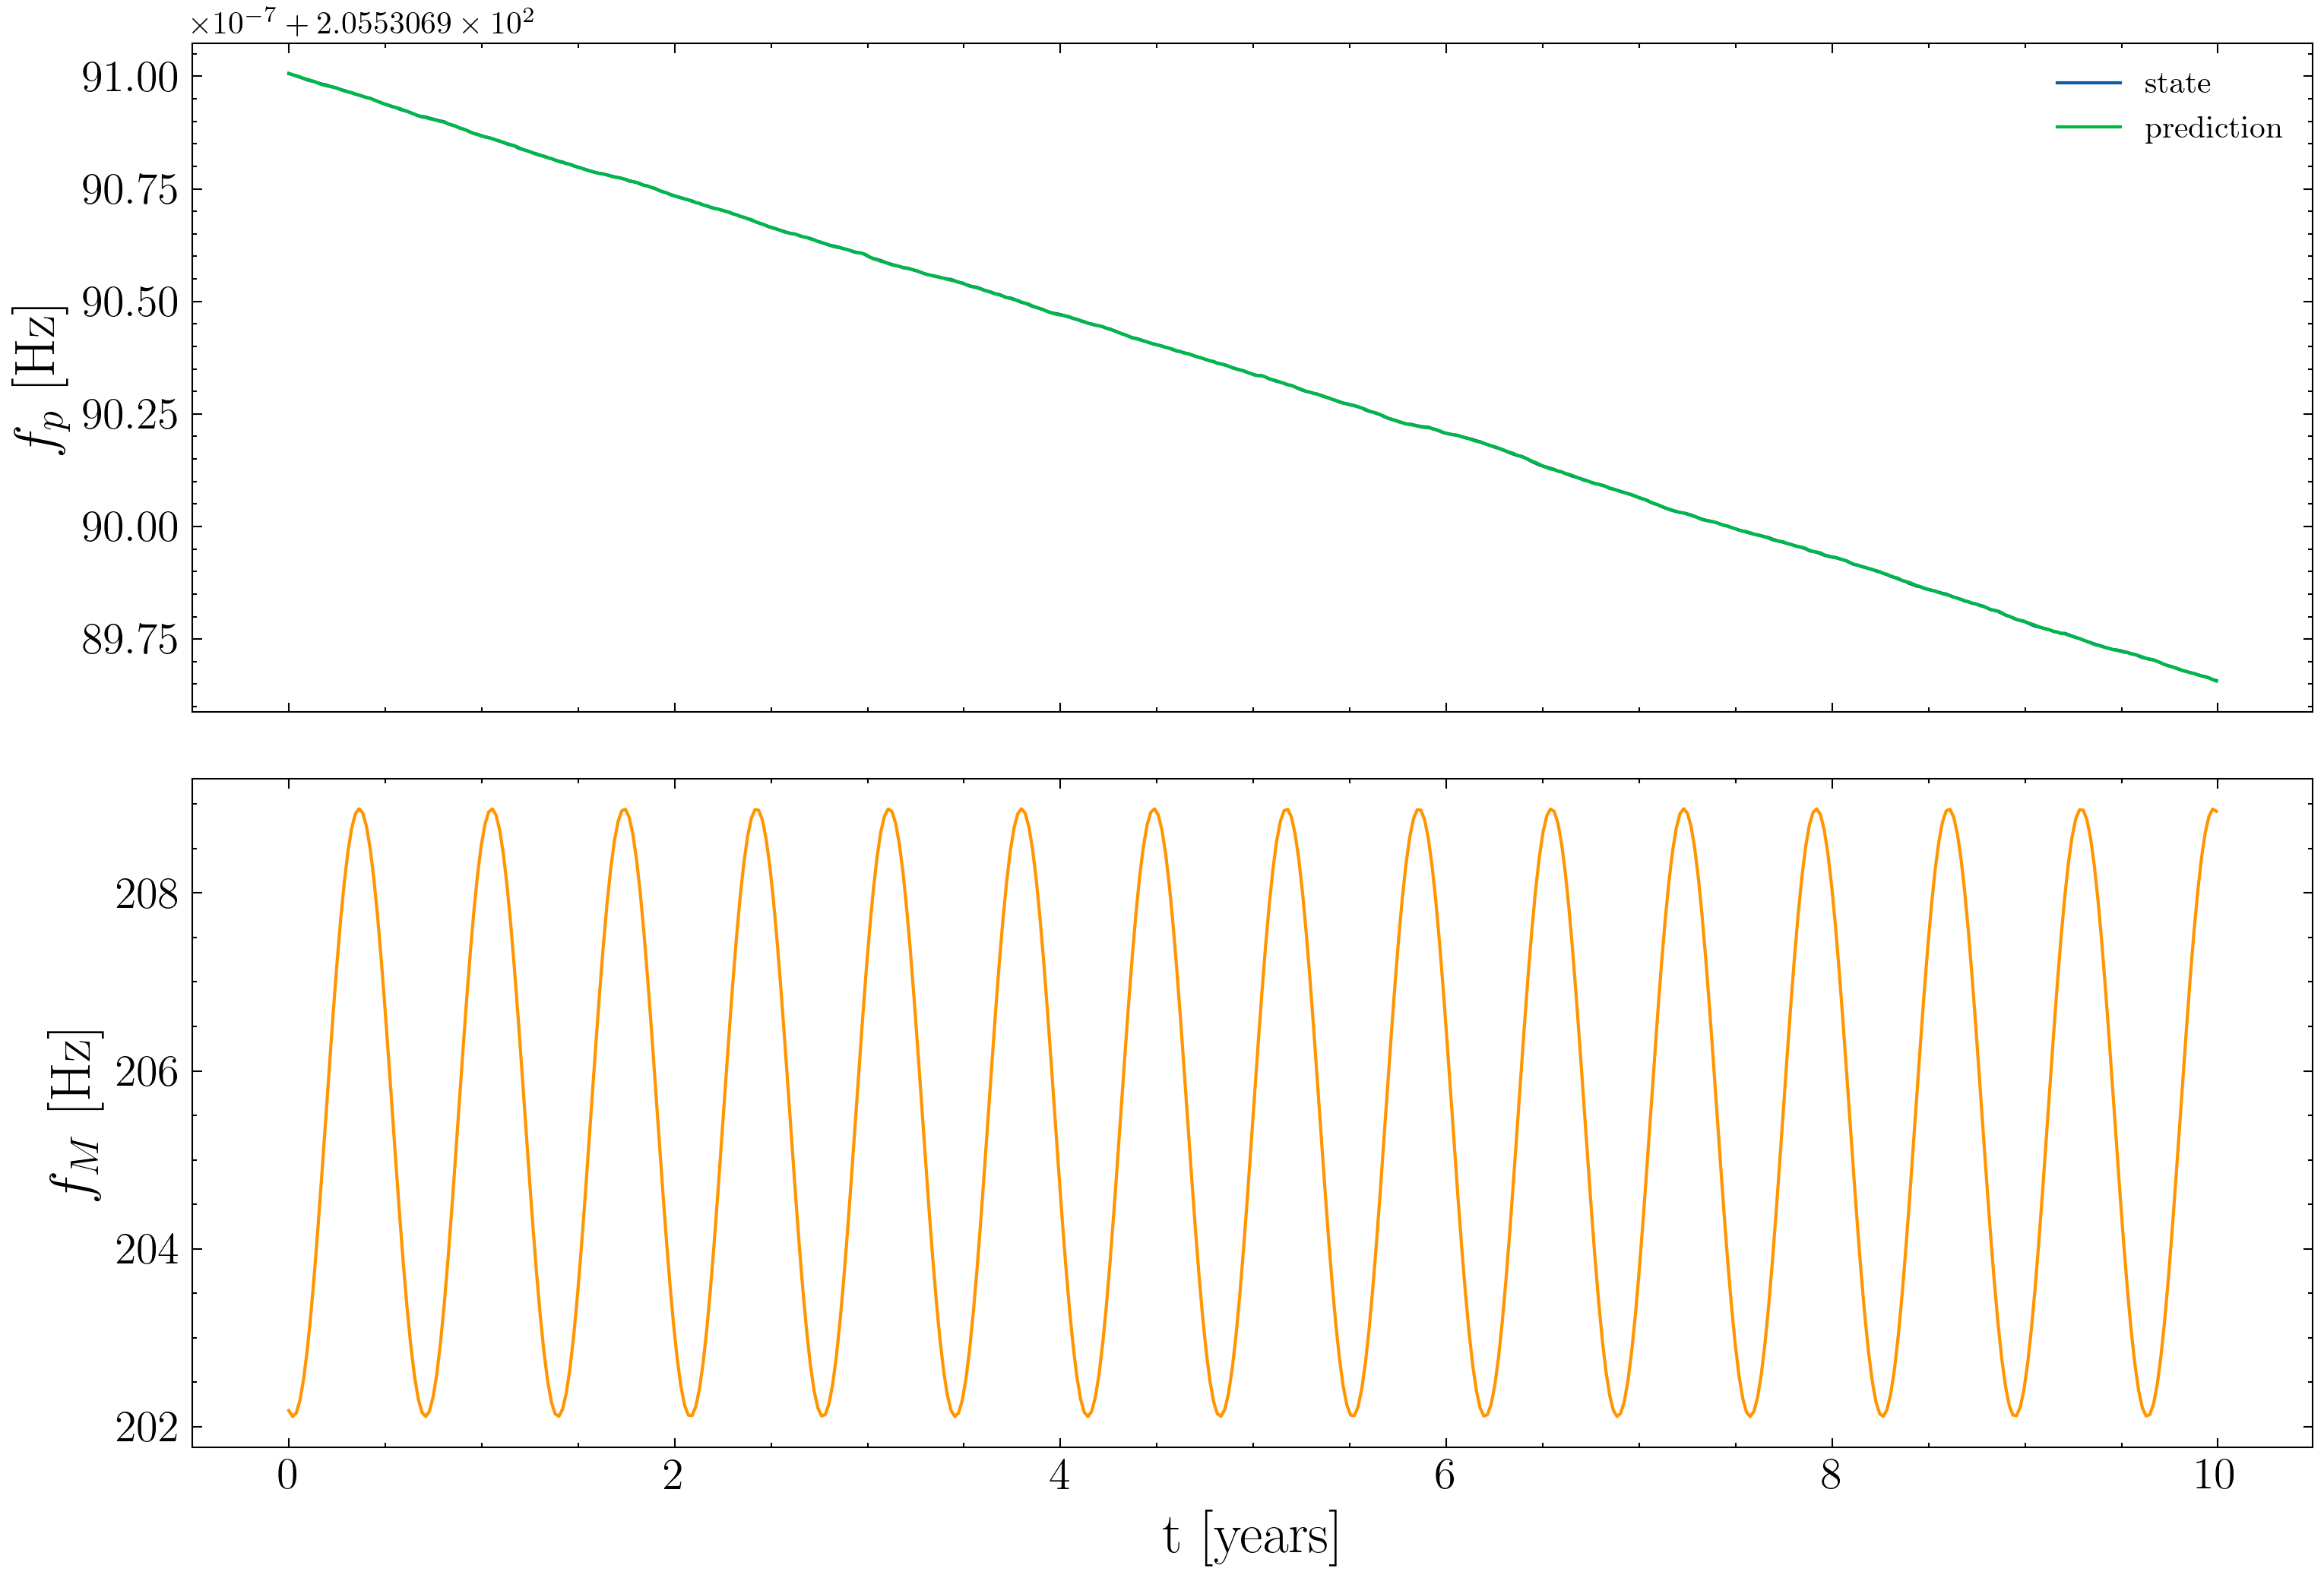
\includegraphics[width=\textwidth]{images/KF1}
		\caption{Using correct parameters}
		\label{fig:6MB_BFS}
	\end{subfigure}
	\hfill
	\begin{subfigure}[b]{1\columnwidth}
		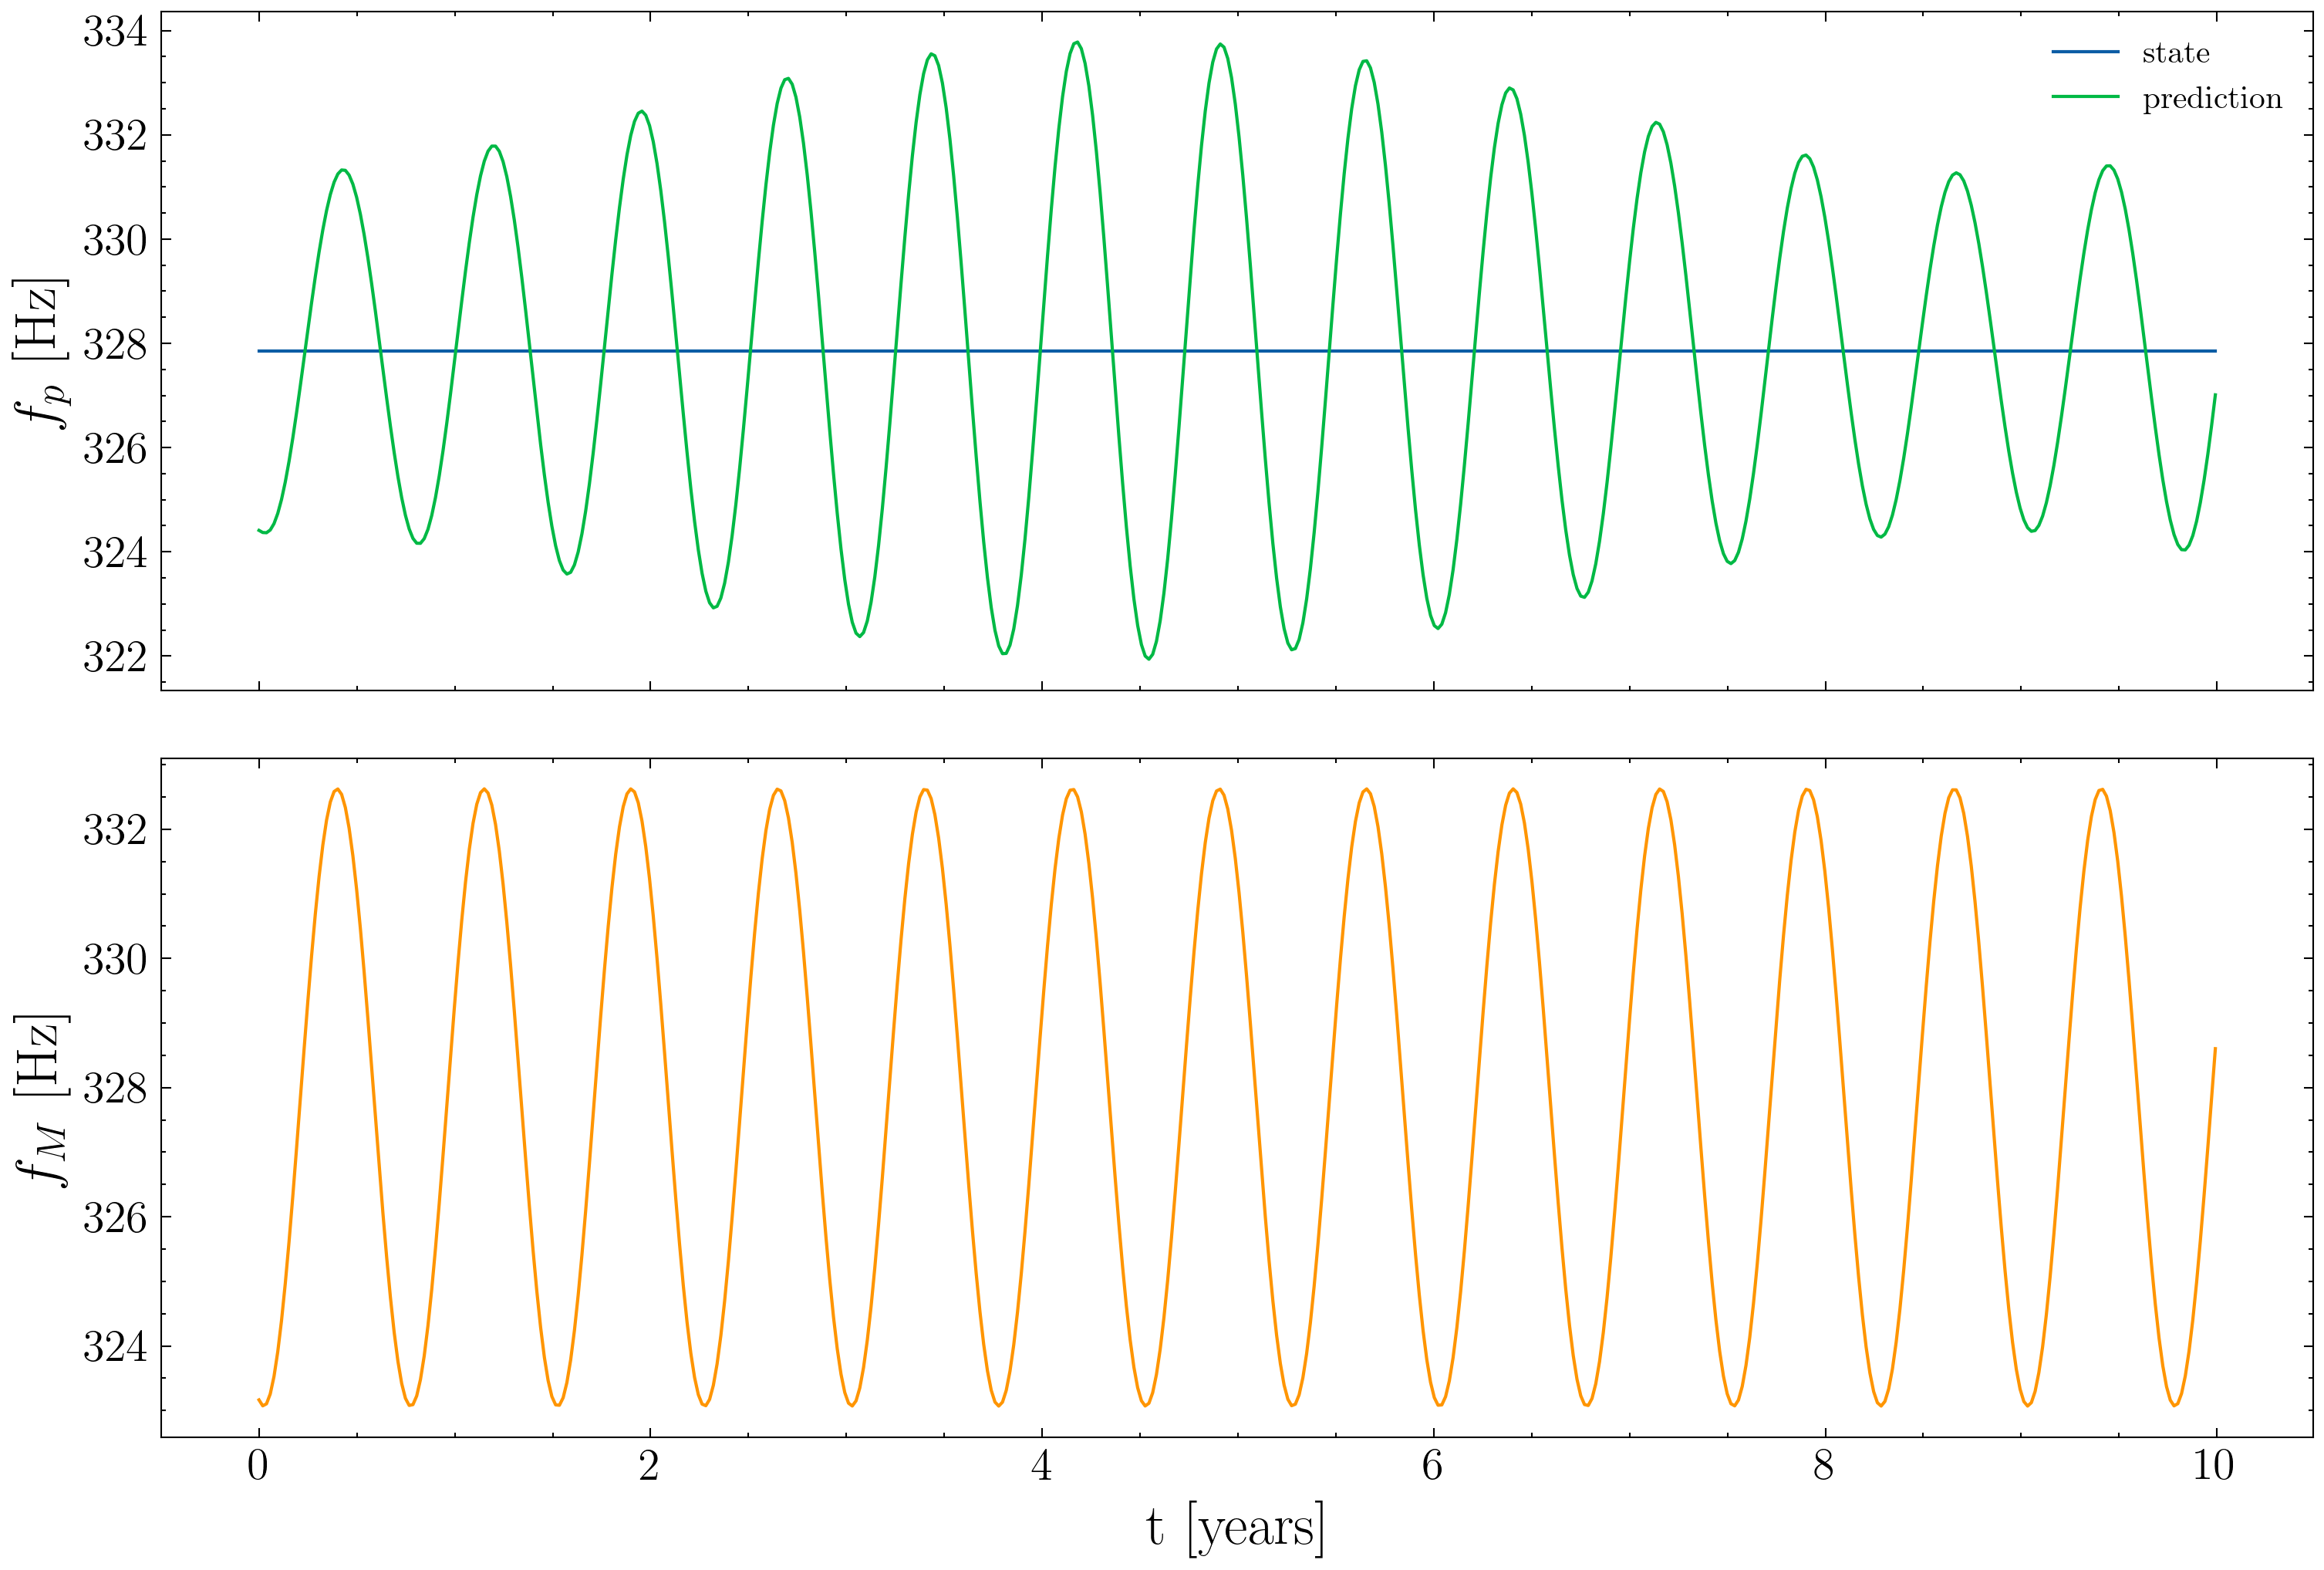
\includegraphics[width=\textwidth]{images/KF2}
		\caption{Using incorrect parameters}
		\label{fig:25MB_bfs}
	\end{subfigure}
	\caption{Application of a Kalman filter to recover the intrinsic frequency states (top panels) given a measured frequency signal (bottom panels) which has been modulated by the presence of a gravitational wave. In the case where the parameters of the filter are accurate (subfigure (a)) the underlying states are also recovered accurately. Conversely, when the parameters fed to the filter are inaccurate (subfigure (b)) the filter cannot recover the state. \textcolor{red}{TK: this needs to be just one stacked figure.}}
	\label{fig:four figures}
\end{figure*}

The Kalman filter \citep{Kalman1} is an algorithm for recovering the most likely evolution of a set of system state variables, $\boldsymbol{X}$ given some noisy measurements $\boldsymbol{Y}$. It is a common technique in signal processing that has been applied successfully in neutron star astrophysics \citep[e.g.][]{Meyers2021,Melatos2023}. In this work we use the linear Kalman filter which assumes a linear relation between $\boldsymbol{X}$ and $\boldsymbol{Y}$. Whilst the measurement equation, Eq. \ref{eq:measurement}, is non-linear in the static parameters it is linear in the state and measurement variables, $f_{\rm p}^{(n)}$ and $f_{\rm m}^{(n)}$ respectively. Extension to non-linear problems is straightforward using either an extended Kalman filter \citep{zarchan2000fundamentals}, the unscented Kalman filter \citep{882463van} or the particle filter \citep{Simon10}. \newline 








The full set of Kalman recursions is presented in Appendix \ref{sec:kalman}. At each discrete timestep $i = 1, ... , M$, the Kalman filter returns an estimate of the state variables, $\hat{\boldsymbol{X}}_i$, and the covariance of those estimates $\boldsymbol{P}_i$. The filter tracks the error in its predictions of $\boldsymbol{X}_i$ by projecting the state predictions back into measurement space, $\hat{\boldsymbol{X}}_i \mapsto \hat{\boldsymbol{Y}}_i$, via the measurement equation. The measurement predictions can then be compared aganst the true observed noisy measurements to get a residual $\boldsymbol{\epsilon}_i = \boldsymbol{Y}_i  - \hat{\boldsymbol{Y}}_i$, sometimes termed the ``innovation". The Kalman filter also calculates the uncertainty in $\boldsymbol{\epsilon}_i$ via the innovation covariance $\boldsymbol{S}_i = \langle \boldsymbol{\epsilon}_i \boldsymbol{\epsilon}_i^{\intercal} \rangle$. The Gaussian log-likelihood can then be calculated at each timestep,
\begin{eqnarray}
	\log \mathcal{L}_i =  -\frac{1}{2} \left (N \log 2 \pi + \log  \left | \boldsymbol{S}_i \right | + \boldsymbol{\epsilon}_i^{\intercal} \boldsymbol{S}_i^{-1}  \boldsymbol{\epsilon}_i \right )
\end{eqnarray}
with the total log-likelihood the sum over all timesteps, i.e. 
\begin{eqnarray}
	\log \mathcal{L} =  \sum_{i=1}^{i=M} \log \mathcal{L}_i  \label{eq:likelihood}
\end{eqnarray}
The likelihood $\mathcal{L}$, along $\hat{\boldsymbol{X}}$ and $\hat{\boldsymbol{Y}}$, are functions of the static parameters of the model, $\bar{\theta}$. If the estimates of the system parameters, $\hat{\theta}$, that we pass to the Kalman filter are close to the true underlying parameters then the error in $\hat{\boldsymbol{X}}$, $\hat{\boldsymbol{Y}}$ is minimized and $\mathcal{L}$ is maximised. This is illustrated in Figure \ref{fig:6MB_BFS}; given a data timeseries of the measured pulsar frequency the Kalman filter is able to recover the hidden state evolution with high fidelity. Conversely, if $\hat{\theta}$ is not close to $\bar{\theta}$ then the filter is unable to recover the state evolution. This is demonstrated in Figure \ref{fig:25MB_bfs} where the failure of the filter to track the hidden state is evident. 


\subsection{Nested Sampling}\label{sec:nested_sampling}

We can use the likelihood returned by the Kalman filter, Eq \ref{eq:likelihood}, in conjunction with likelihood-based inference methods to estimate the posterior distribution of $\bar{\theta}$ by Bayes' Rule,
\begin{equation}
	p(\bar{\theta} | \boldsymbol{Y}) = \frac{\mathcal{L} \cdot \pi(\theta)}{\mathcal{Z}}
\end{equation}
where $\pi(\theta)$ is the prior distribution on $\bar{\theta}$ and $\mathcal{Z}$ is the marginalised likelihood, or evidence
\begin{equation}
	\mathcal{Z} = \int \mathcal{L} \pi (\theta) d \theta \label{eq:model_evidence}
\end{equation}
In order to estimate the posterior distribution and the model evidence we use nested sampling \citep[NS,][]{Skilling}. Nested sampling is an integration algorithm used for evaluating marginalised likelihood integrals, of the form given by Eq. \ref{eq:model_evidence}, that also returns samples from the posterior $p(\bar{\theta} | \boldsymbol{Y})$. The primary advantage of nested sampling is the ability to compute this evidence integral, which is key for model selection, and proves difficult without considerable extra cost for the usual Markov Chain Monte Carlo (MCMC) approaches. Nested sampling is also typically less computationally intensive than MCMC and can handle multi-modal problems \citep{Ashton2022}. For these reasons, it has enjoyed widespread adoption in the physical sciences, particularly within the cosmological community \citep{Mukherjee2006,Feroz2008,Handley2015}, but has also commonly been applied in astrophysics \citep{UltraNest2021}, particle physics \citep{proceedings2019033014} and materials science \citep{2009arXiv0906materials}. Within this work we exclusively use nested sampling for Bayesian parameter estimation and model selection. \newline 


\noindent Multiple nested sampling libraries exist. For gravitational astrophysics it is common to use the dynesty sampler CITE, via the Bilby gravitational wave inference library and we continue to follow this precedent. 
\textcolor{red}{TK: update text here from other version}


\subsection{Model selection}\label{sec:model_selection}
The evidence integral returned by nested sampling is the probability of the data $\boldsymbol{Y}$ given a particular model $\mathcal{M}$. This enables us to compare competing models via a Bayes factor,
\begin{equation}
	\beta = \frac{\mathcal{Z}(\mathcal{M}_1)}{\mathcal{Z}(\mathcal{M}_0)}
\end{equation}
where the subscript index identifies a particular model. Throughout this work we take $\mathcal{M}_1$ to be the complete model defined in Section \ref{sec:model}. $\mathcal{M}_0$ is our null model that assumes there is no GW in the data. This is equivalent to setting $g^{(n)}(t)$ from Equation \ref{eq:g_func}, \ref{eq:g_func_trig} $= 1$. The Bayes factors we quote in this paper therefore quantify whether the data shows evidence for a GW compared to no GW.


\section{Tests with synthetic data} \label{sec:testing}




We go on to discuss our choice of pulsars to make up our PTA in Section \ref{sec:pta_pulsars}, before deploying these techniques in Sections \ref{sec:param_estimation} , \ref{sec:detection} for parameter estimation and model selection.


\subsection{Practical considerations}

heterodyeing 

pulsar terms 
For now we will consider the measurement noise to be known, although in principle this too could be estimated. 





\subsection{PTA pulsars}\label{sec:pta_pulsars}
\begin{figure}
	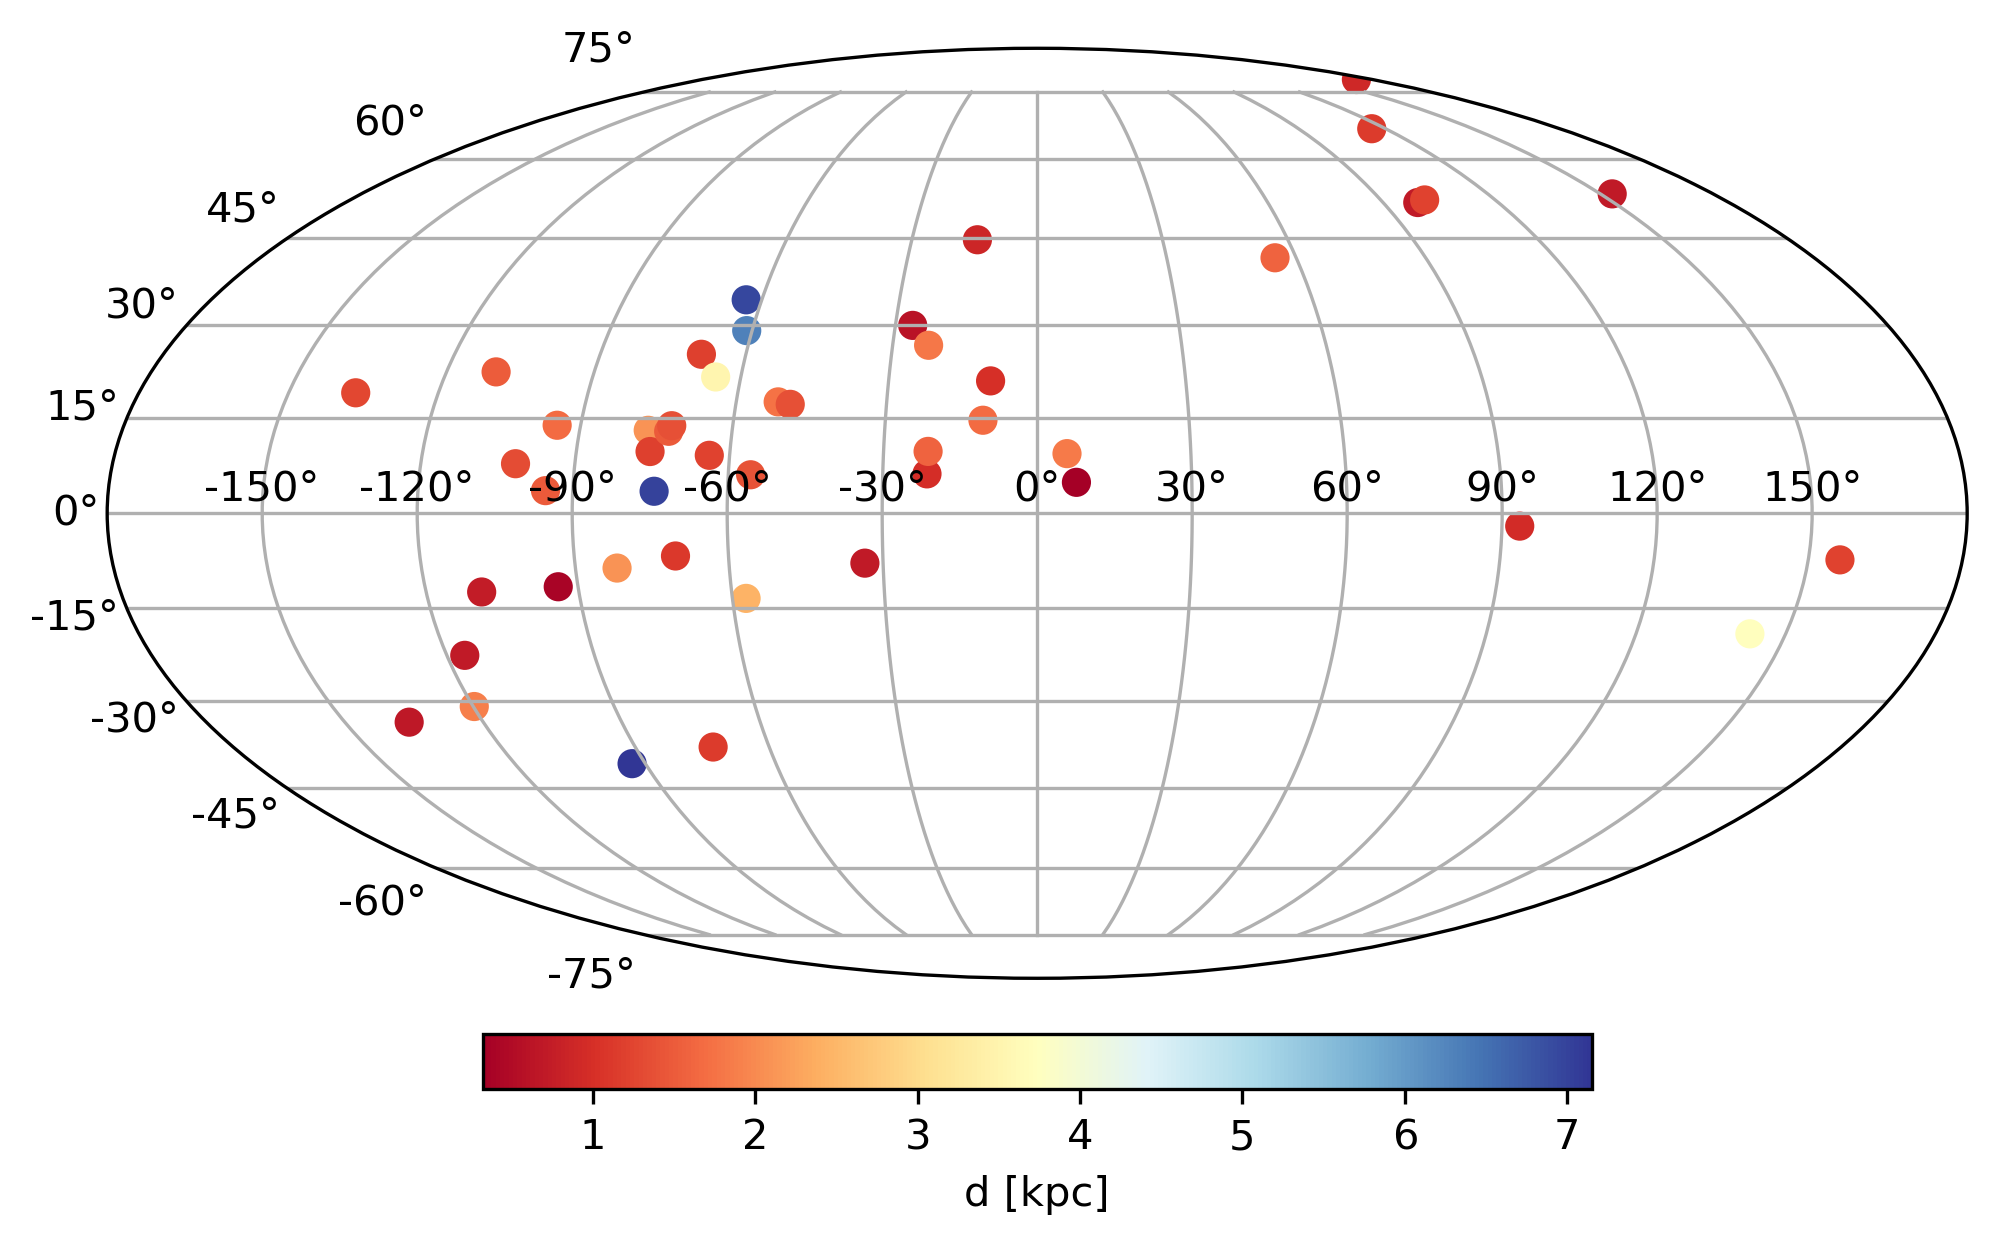
\includegraphics[width=0.8\columnwidth]{images/pulsars}
	\caption{Spatial distribution and distances of NANOGrav pulsars}
	\label{fig:pulsar_distrib}
\end{figure}
\noindent With our Kalman filter and nested sampling techniques in hand, in order to proceed it is necessary to specify a PTA configuration. As discussed, multiple separate PTA detectors exist under the umbrella of the IPTA. Going forward we will take the 47 pulsars that make up the NANOGrav PTA \citep{2020ApJ...905L..34A}. NANOGrav is selected simply as a well-representative example of the typical pulsars that make up a PTA. Our results and formulation are not contingent on the choice of PTA, and naturally extend to other PTAs or PTAs with more pulsars.  \newline 



\noindent Within our state-space formulation, the pulsar evolution is governed by a set of 5 parameters, $\bar{\theta}_{\rm PSR}$ for each pulsar. The parameters $f_{\rm EM} (0) $,$ \dot{f}_{\rm EM} (0)$ and $d$ are well specified via existing pulsar datasets. We take the frequency and frequency derivative as returned from the pulsar datasets to simply be the values now at $t=0$. The pulsar distances are also known, though less well constrained. Going forward we take the distances retuned from the datasets as the true values of the pulsars that make up our synthetic PTA. The specification of $\gamma$ and $\sigma$ are more involved. $\gamma$ specifies an effective timescale of reversion to the mean \textcolor{red}{TK: Need some discussion and though on how to choose these two parameters to be astrophysically reasonable c.f. A. Vargas}


\subsection{Parameter estimation}\label{sec:param_estimation}
We are now in a position to try to infer the parameters of a GW system. We take our NANOGrav PTA and create a synthetic noisy dataset using the parameters described in Table \ref{tab:toy_example_parameters}.
\begin{table}
	\centering
	\begin{tabular}{lc}
		Parameter & Value  \\
		\hline
		$\omega$       & $5 \times 10^{-7}$  \\
		$\alpha$          & $1.0$  \\
		$\delta$              & $1.0$   \\
		$\psi$              & $2.50$  \\
		$\iota$             & $1.0$  \\
		$\Phi_0$          & $0.20$  \\
		$h$ & 1e-2 \\
		$\sigma_{\rm p}$ & $10^{-13}$ \\
		$\sigma_{\rm m}$ & $10^{-10}$ \\
		$T_{obs}$ & 10 \text{ years} \\
		$\Delta t$ & 7 \text{ days} \\
		\hline
	\end{tabular}
	\caption{GW parameters used for generating synthetic data. There is nothing special about these parameters - they are just chosen arbitrarily.}
	\label{tab:toy_example_parameters}
\end{table}
\noindent Given this synthetic data, we can try to use our KF + NS approach to recover some of the parameters. The results for inference on 5 parameters, $\omega. \Phi_0, \psi, \iota, h$ are shown in Fig \ref{fig:corner2}. \textcolor{red}{TK: likelihood plots for each parameter could also be of interest to include here? Need to expand this section greatly for more astrophysical systems and more unknown parameters}
%\begin{figure*}
%	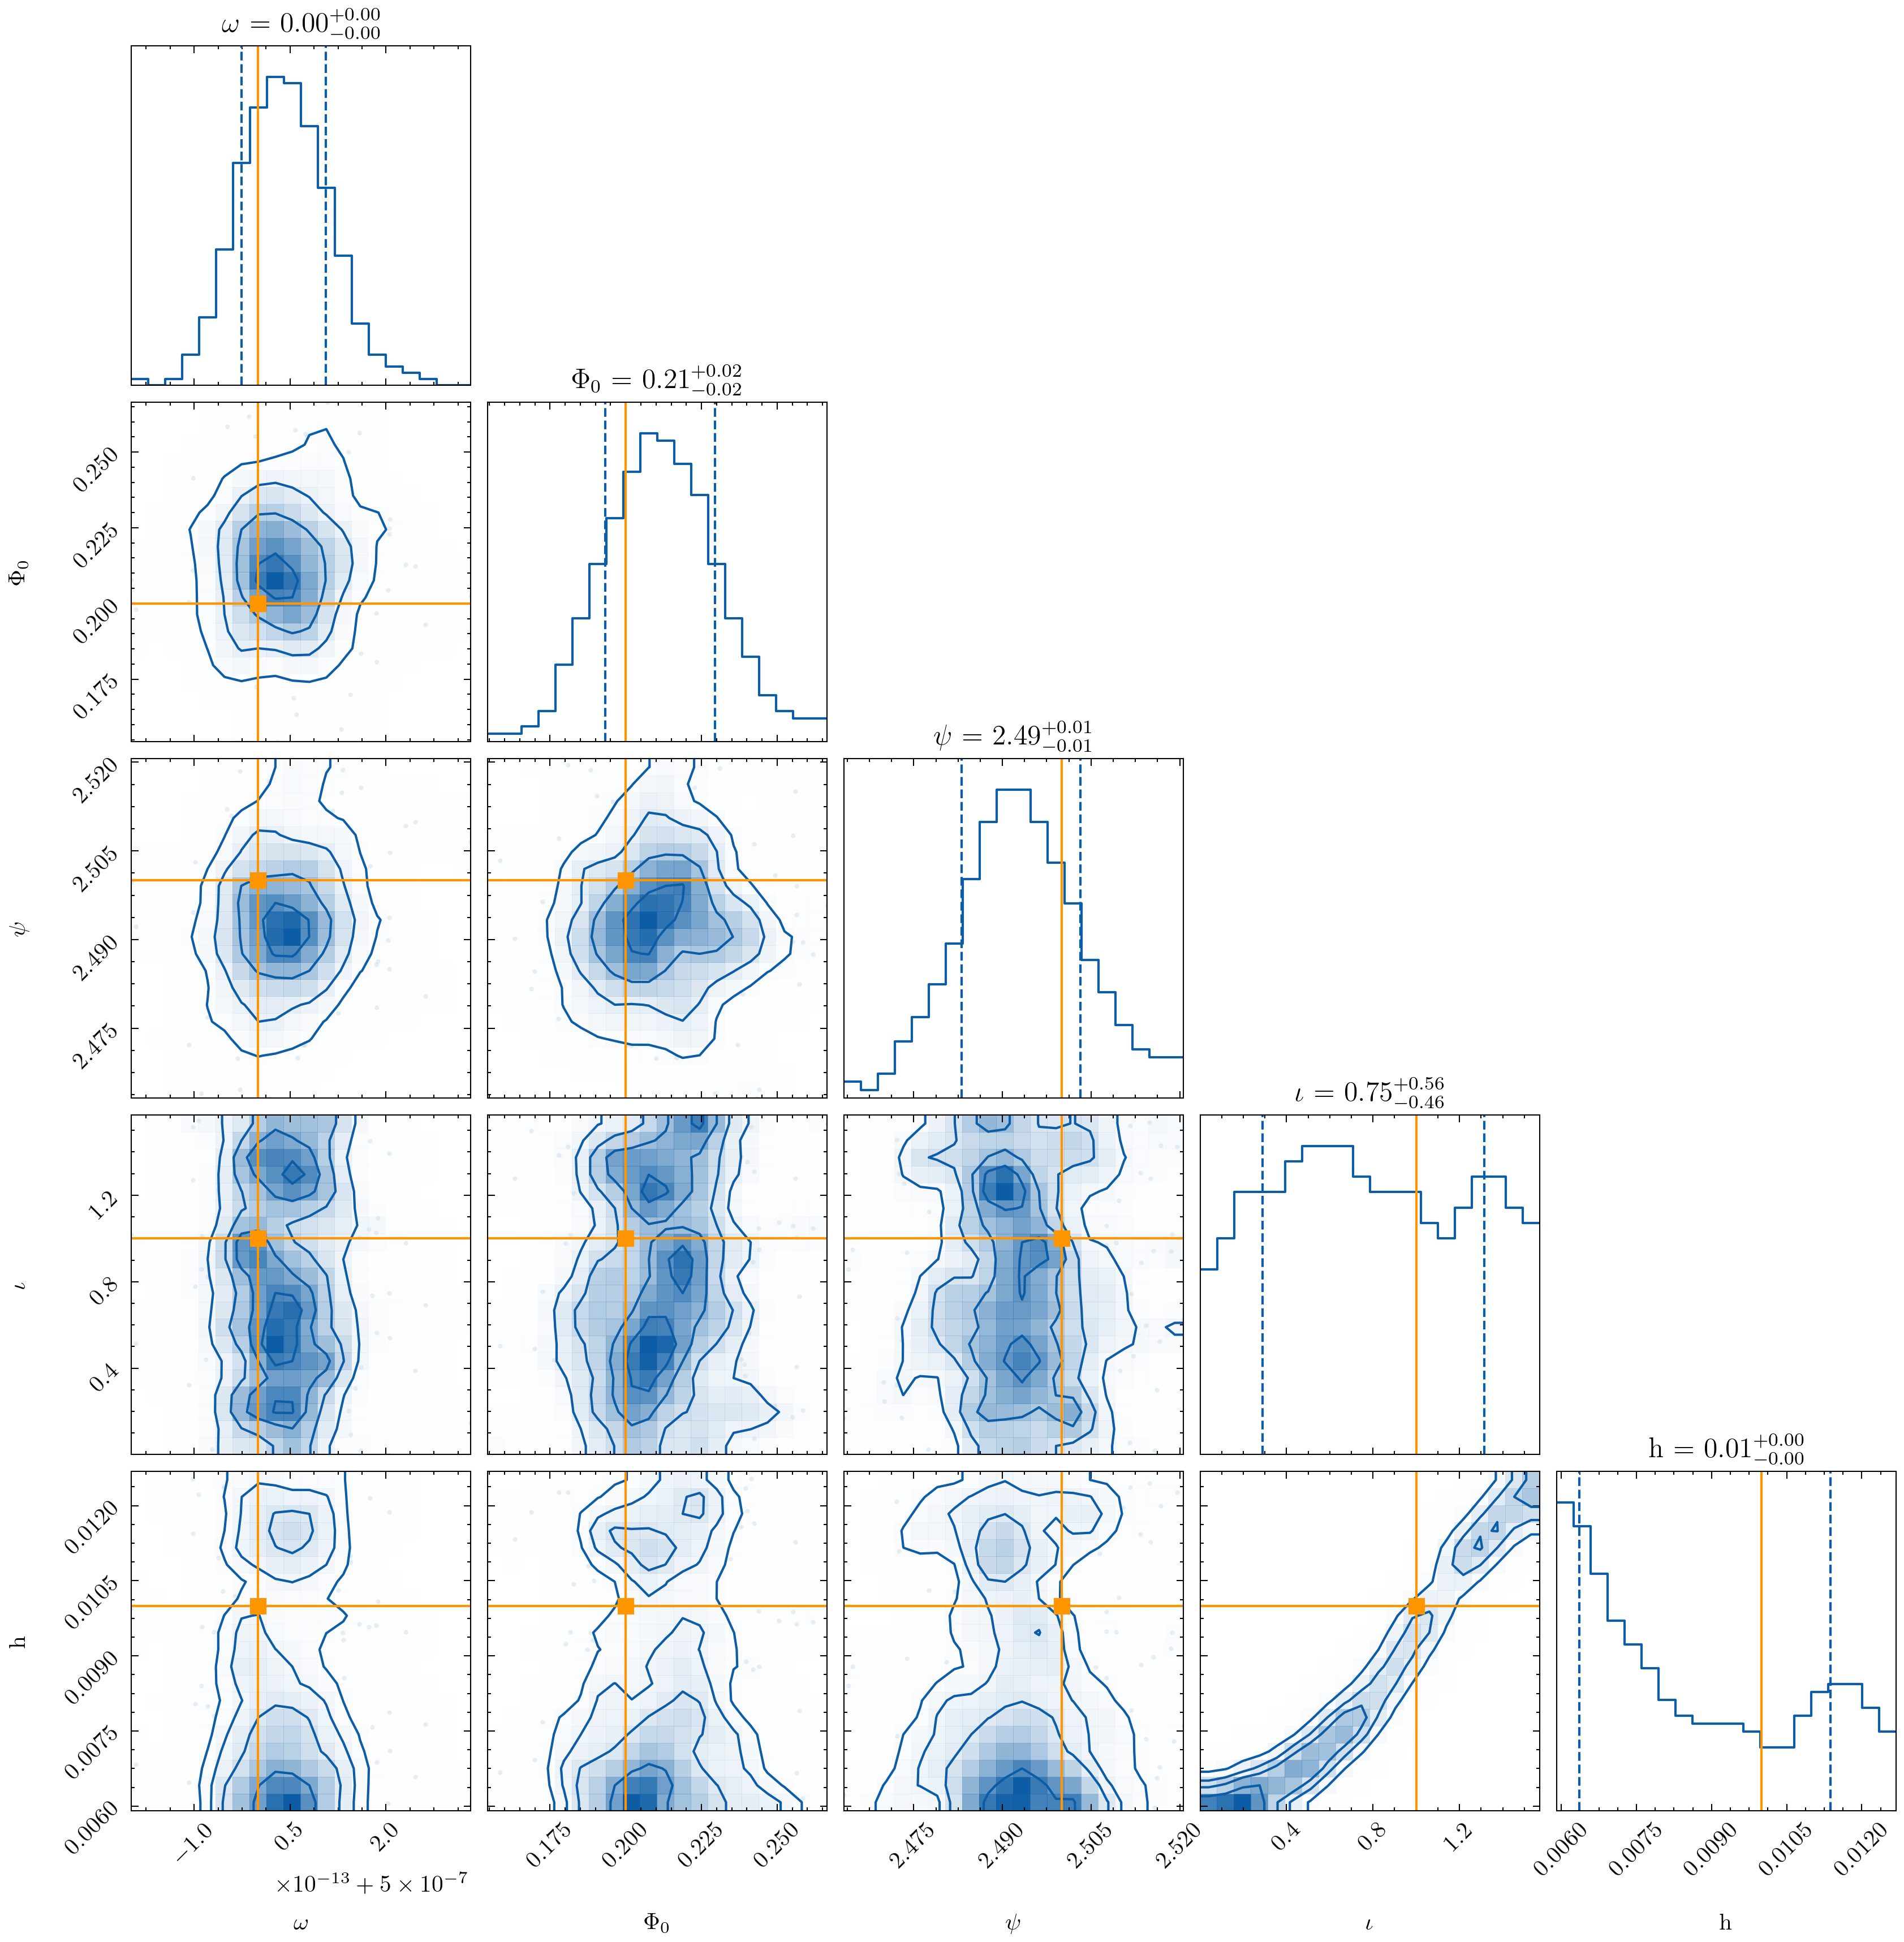
\includegraphics[width=0.8\textwidth]{images/corner_example}
%	\caption{Example corner plot. Aside: for this run the $\sigma_p$ value fed to the filter is different from that used to generate the data.}
%	\label{fig:corner}
%\end{figure*}



\begin{figure*}
	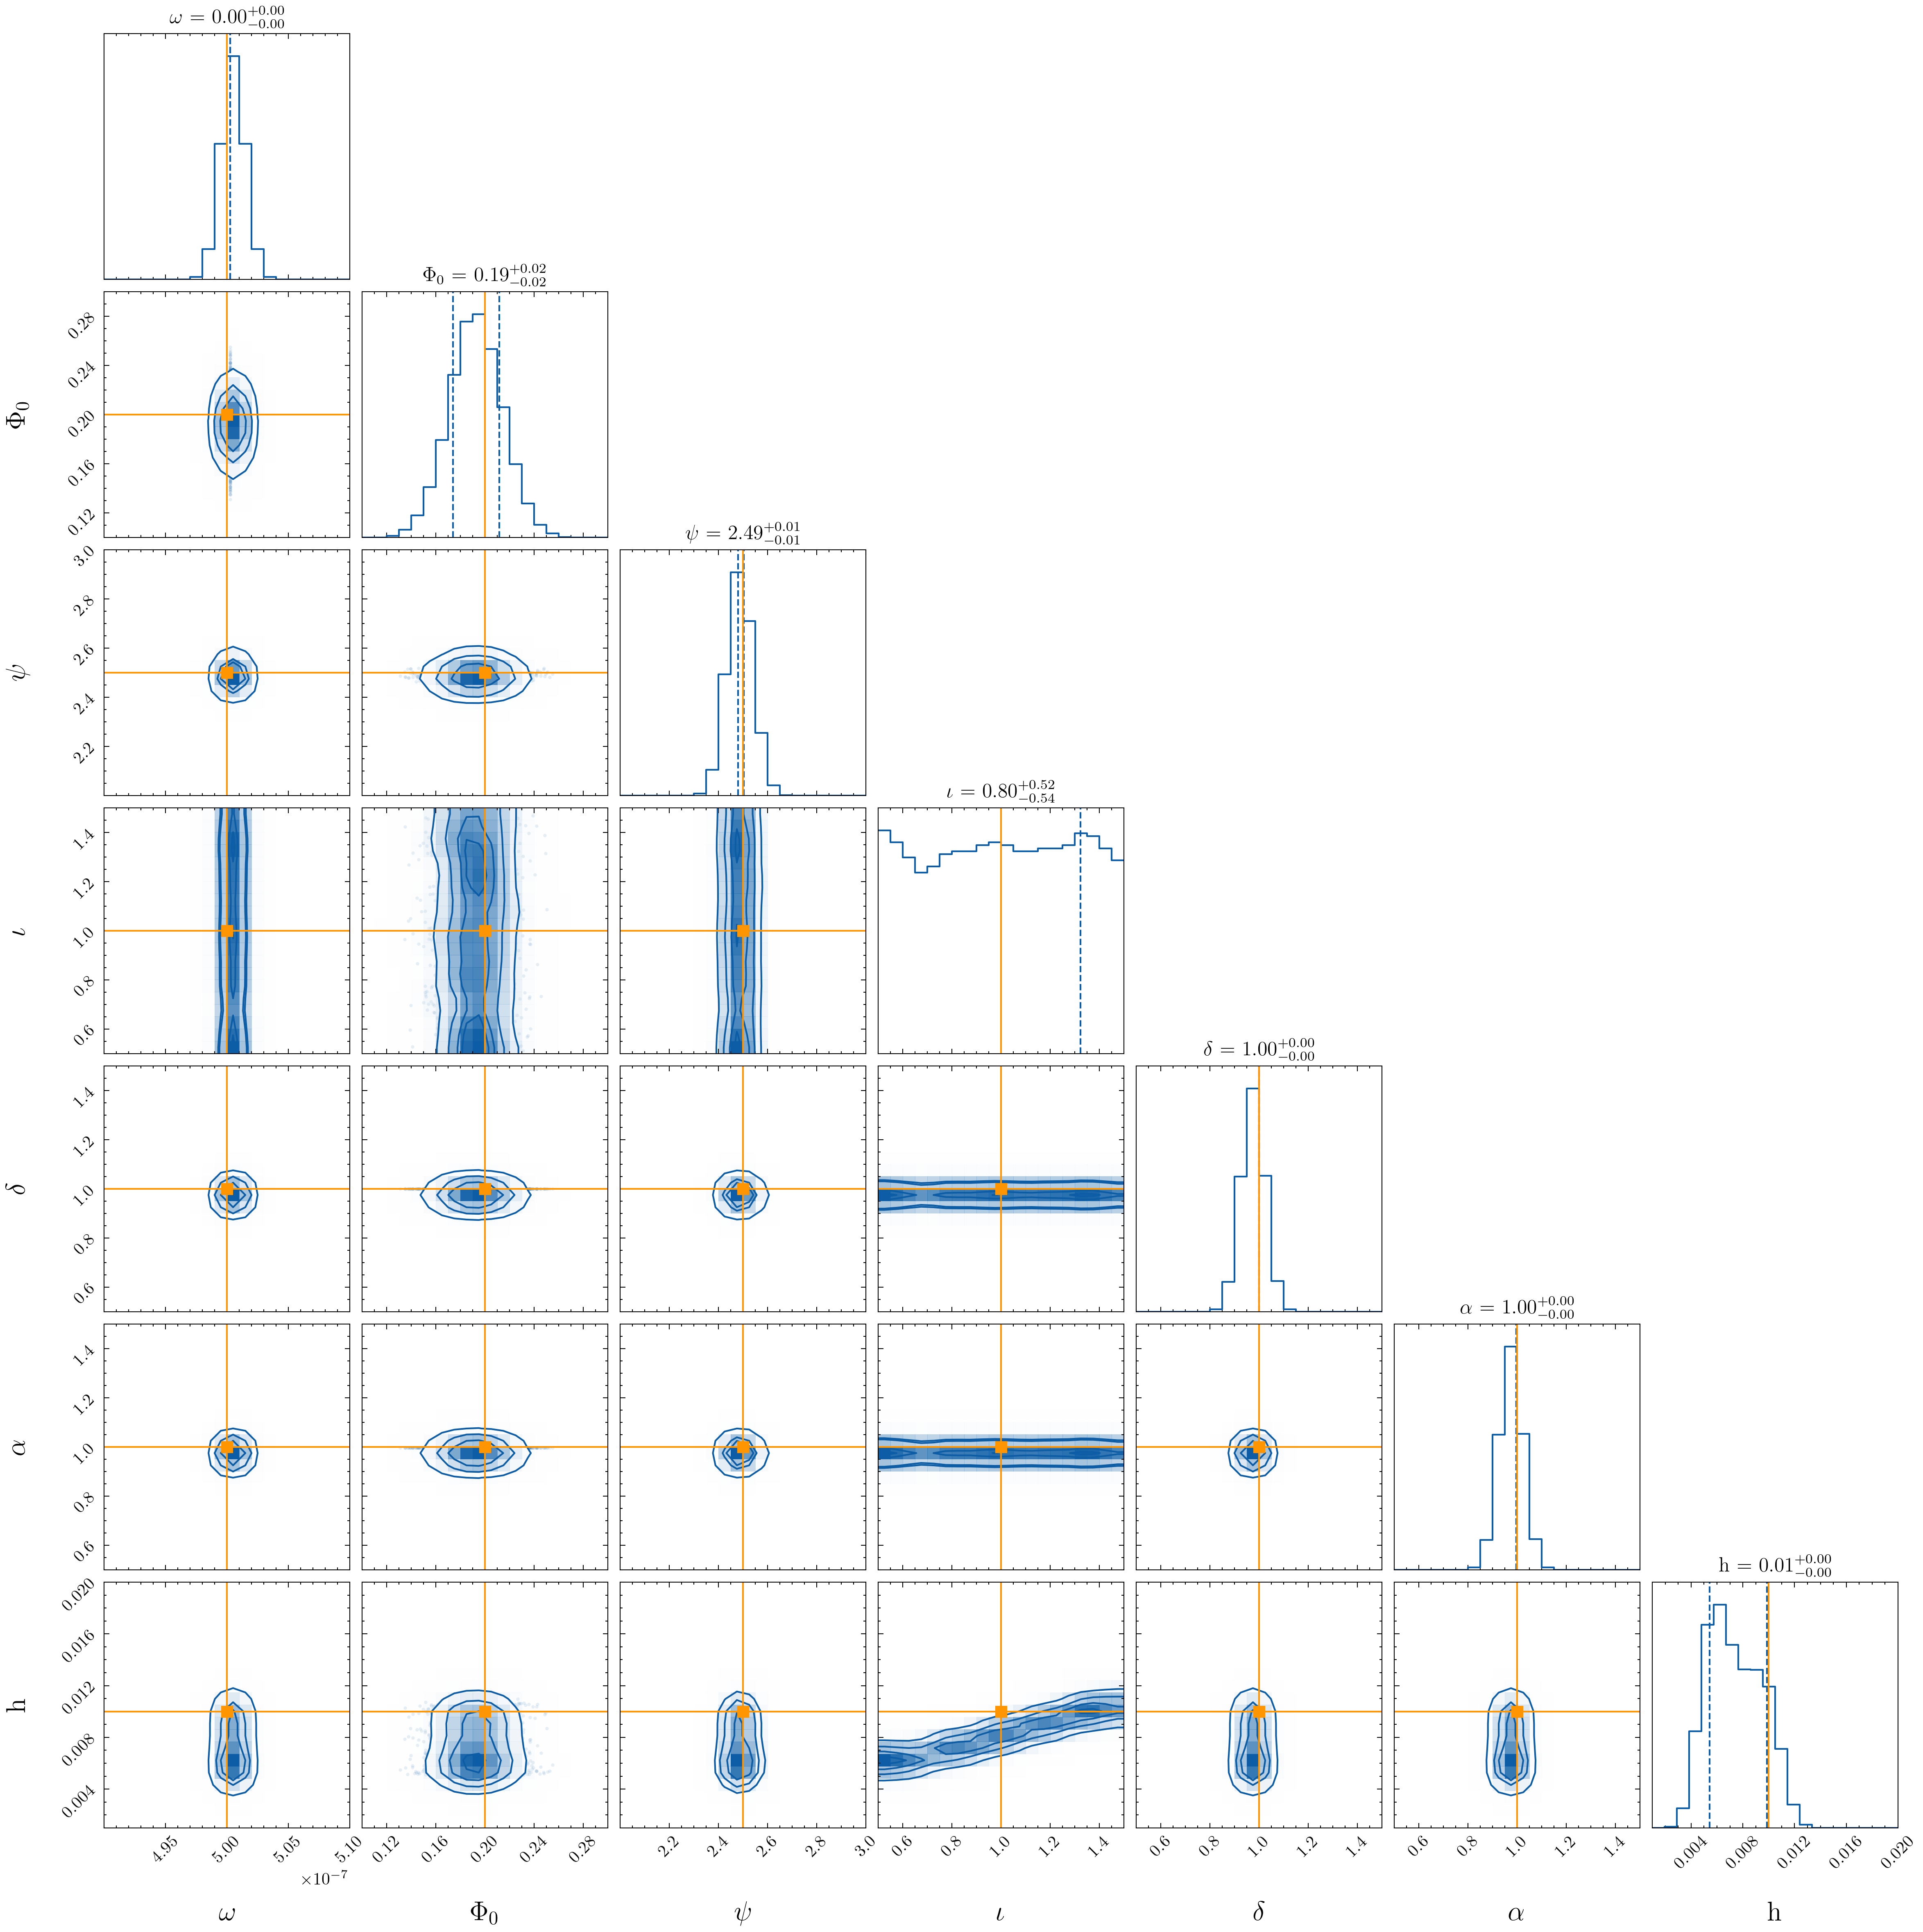
\includegraphics[width=0.8\textwidth]{images/canonical_example}
	\caption{Example corner plot. Aside: for this run the $\sigma_p$ value fed to the filter is different from that used to generate the data.}
	\label{fig:corner2}
\end{figure*}

\subsection{Detection}\label{sec:detection}

In addition to estimating the parameters of the system, we are also interested in how detectable a GW is using PTA + state space method. We can use our state-space tools  to try to solve the problem of GW detection with a PTA i.e. \textit{"Is there evidence of a GW in my data?"}We can frame this as a model selection procedure where we have two models/hypotheses:

\begin{itemize}
\item Null Model, $M_0$. There is no GW in the data. In this case the measurement model of the Kalman filter simply returns the frequency states i.e. $g(t,\theta)= 0$
\item Alternative model, $M_1$. There is a GW in the data. The measurement model uses the full expression for $g(t,\theta)$
\end{itemize}



In order to accept the alternative hypothesis $M_1$ over $M_0$ there are two approaches we could take:

\begin{enumerate}
	\item The first is a fully Bayesian search over all the parameters for each model, calculating the evidence for each model and then determining the Bayes ratio. This is perhaps the most consistent way, but it is obviously expensive and at this stage we are keen to explore how detectability varies with e.g. GW strain.
	\item The second method is to recognize that $M_0$ and $M_1$ are hierarchically nested models and we can perform a likelihood ratio test. That is, given the maximum likelihood estimators $\hat{\theta}$ of the true parameters $\theta$, the likelihood of each model can be calculate. These likelihoods are just  point estimates of the Bayes factor numerator/denominators. They can then be compared via the likelihood ratio $\Lambda$. 
\end{enumerate}
Given the cheap cost we proceed with the second method. For the likelihood ratio test we do not perform any kind of maximum likelihood search over the parameters for each of the models. Instead we just artificially set the maximum likelihood estimators to be equal to the true parameters of the system i.e. $\hat{\theta} = \theta$. We assume that any maximum likelihood algorithm would converge to these parameters. This is obviously an oversimplification but will serve our purposes for now. \newline 


\noindent Interpreting the likelihood ratio $\Lambda$ also needs some consideration, since we have to account for the increased model complexity of $M_1$. Bayes factors penalise complexity by construction since one must integrate over a larger parameter space. There are many different ways to do this - fot now we will consider two: Akaike information criterion (AIC) and Wilks Theorem. For the latter, Wilks' Theorem which states that for a large number of samples \footnote{What counts as large? See \url{https://www.osti.gov/servlets/purl/1529145}} the distribution of the test statistic approaches the chi-squared distribution under the null hypothesis i.e. 
\begin{equation}
	2 \log \Lambda \rightarrow \chi^2
\end{equation}
One can then compute $p$-values where the number of degrees of freedom is equal to the difference in the number of parameters of the two models; $M_1$ has 7 extra parameters over $M_0$ corresponding to the 7 parameters of $\bar{\theta}_{\rm GW}$. With 7 degrees of freedom and a target tolerance of 5(1) \% the test statistic is $\sim 14 (18.5)$. \newline 

An alternative approach is to use the AIC which is given by,
\begin{equation}
	\text{AIC} = 2k - 2\log\ \mathcal{L} 
\end{equation}
where $k$ is the number of degrees of freedom. The AIC can be computed for each model and the model with the minimum AIC is preferred. This can be straightforwardly mapped into a relative condition
\begin{equation}
	\log \mathcal{L}_1 - 	\log \mathcal{L}_0 > 7 
\end{equation}
Note this is the same as the Wilks case!

\noindent 





\begin{figure}
	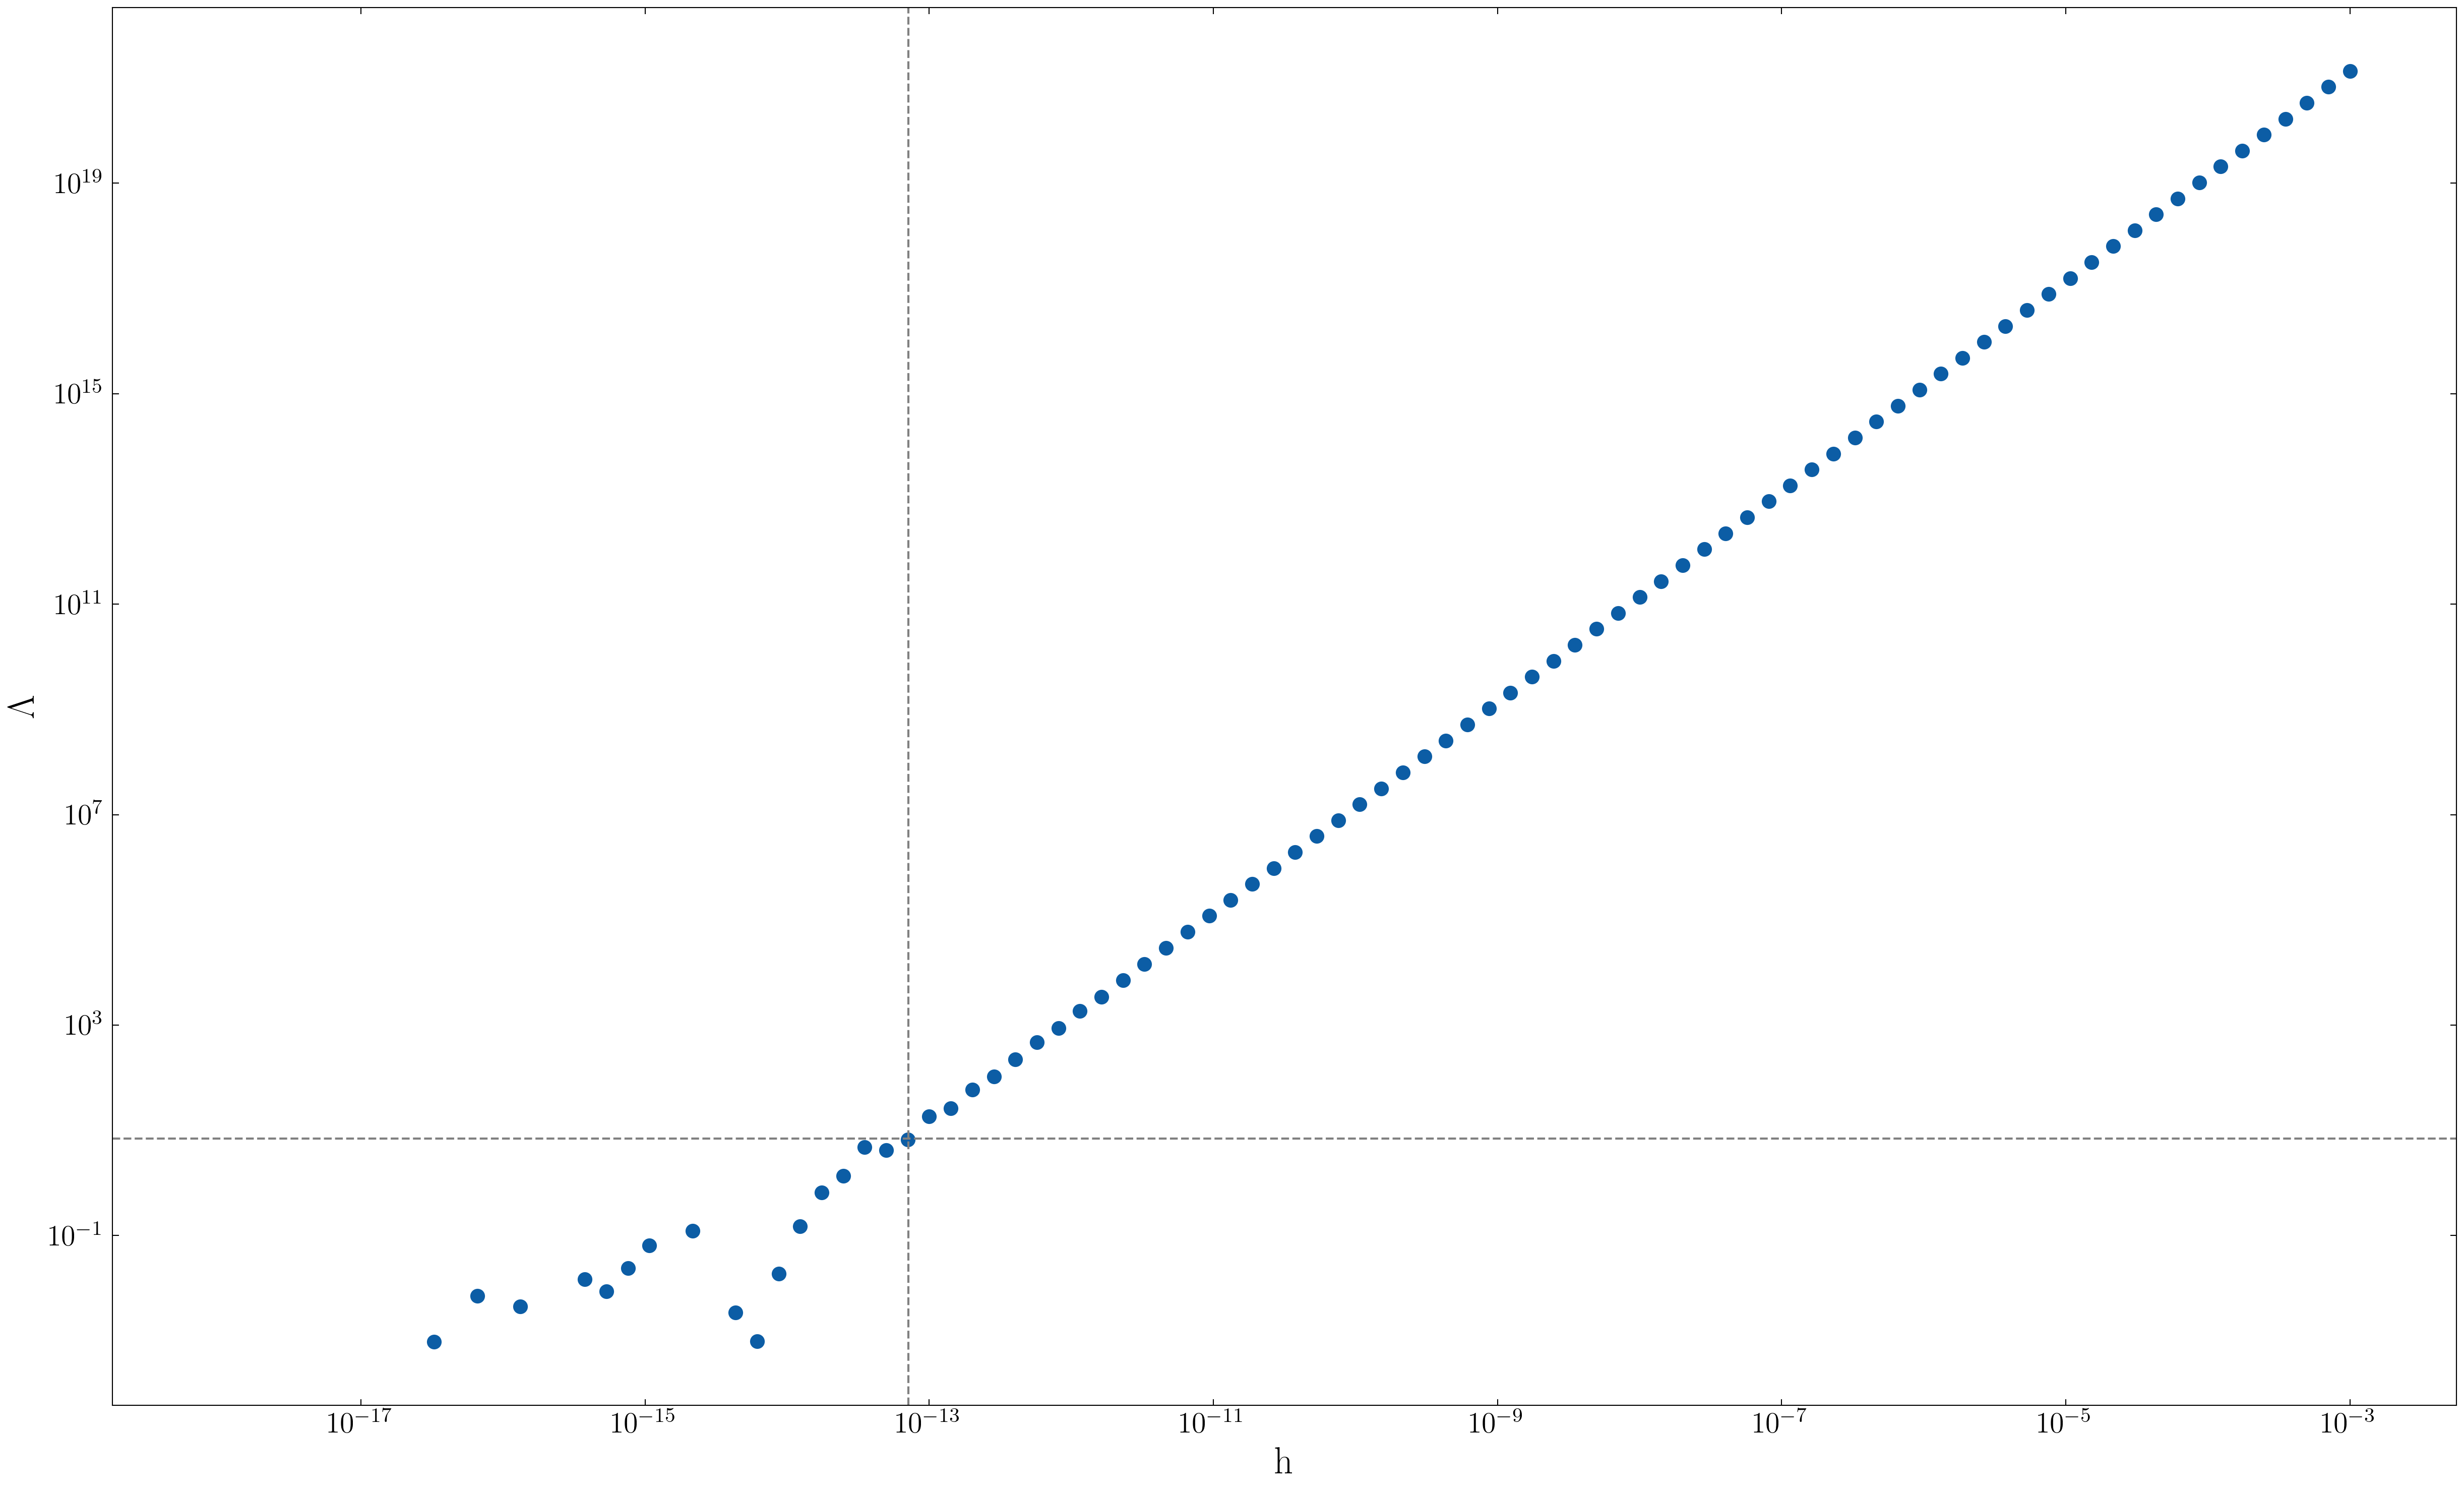
\includegraphics[width=\columnwidth]{images/snr_canonical}
	\caption{Likelihood ratio vs strain for \textit{(a)} full PTA and \textit{(b)} a single randomly chosen pulsar. Horizontal dashed line shows the minimum detectable cutoff, vertical dashed lines are the corresponding GW strains.}
	\label{fig:SNR}
\end{figure}





\begin{figure*}
	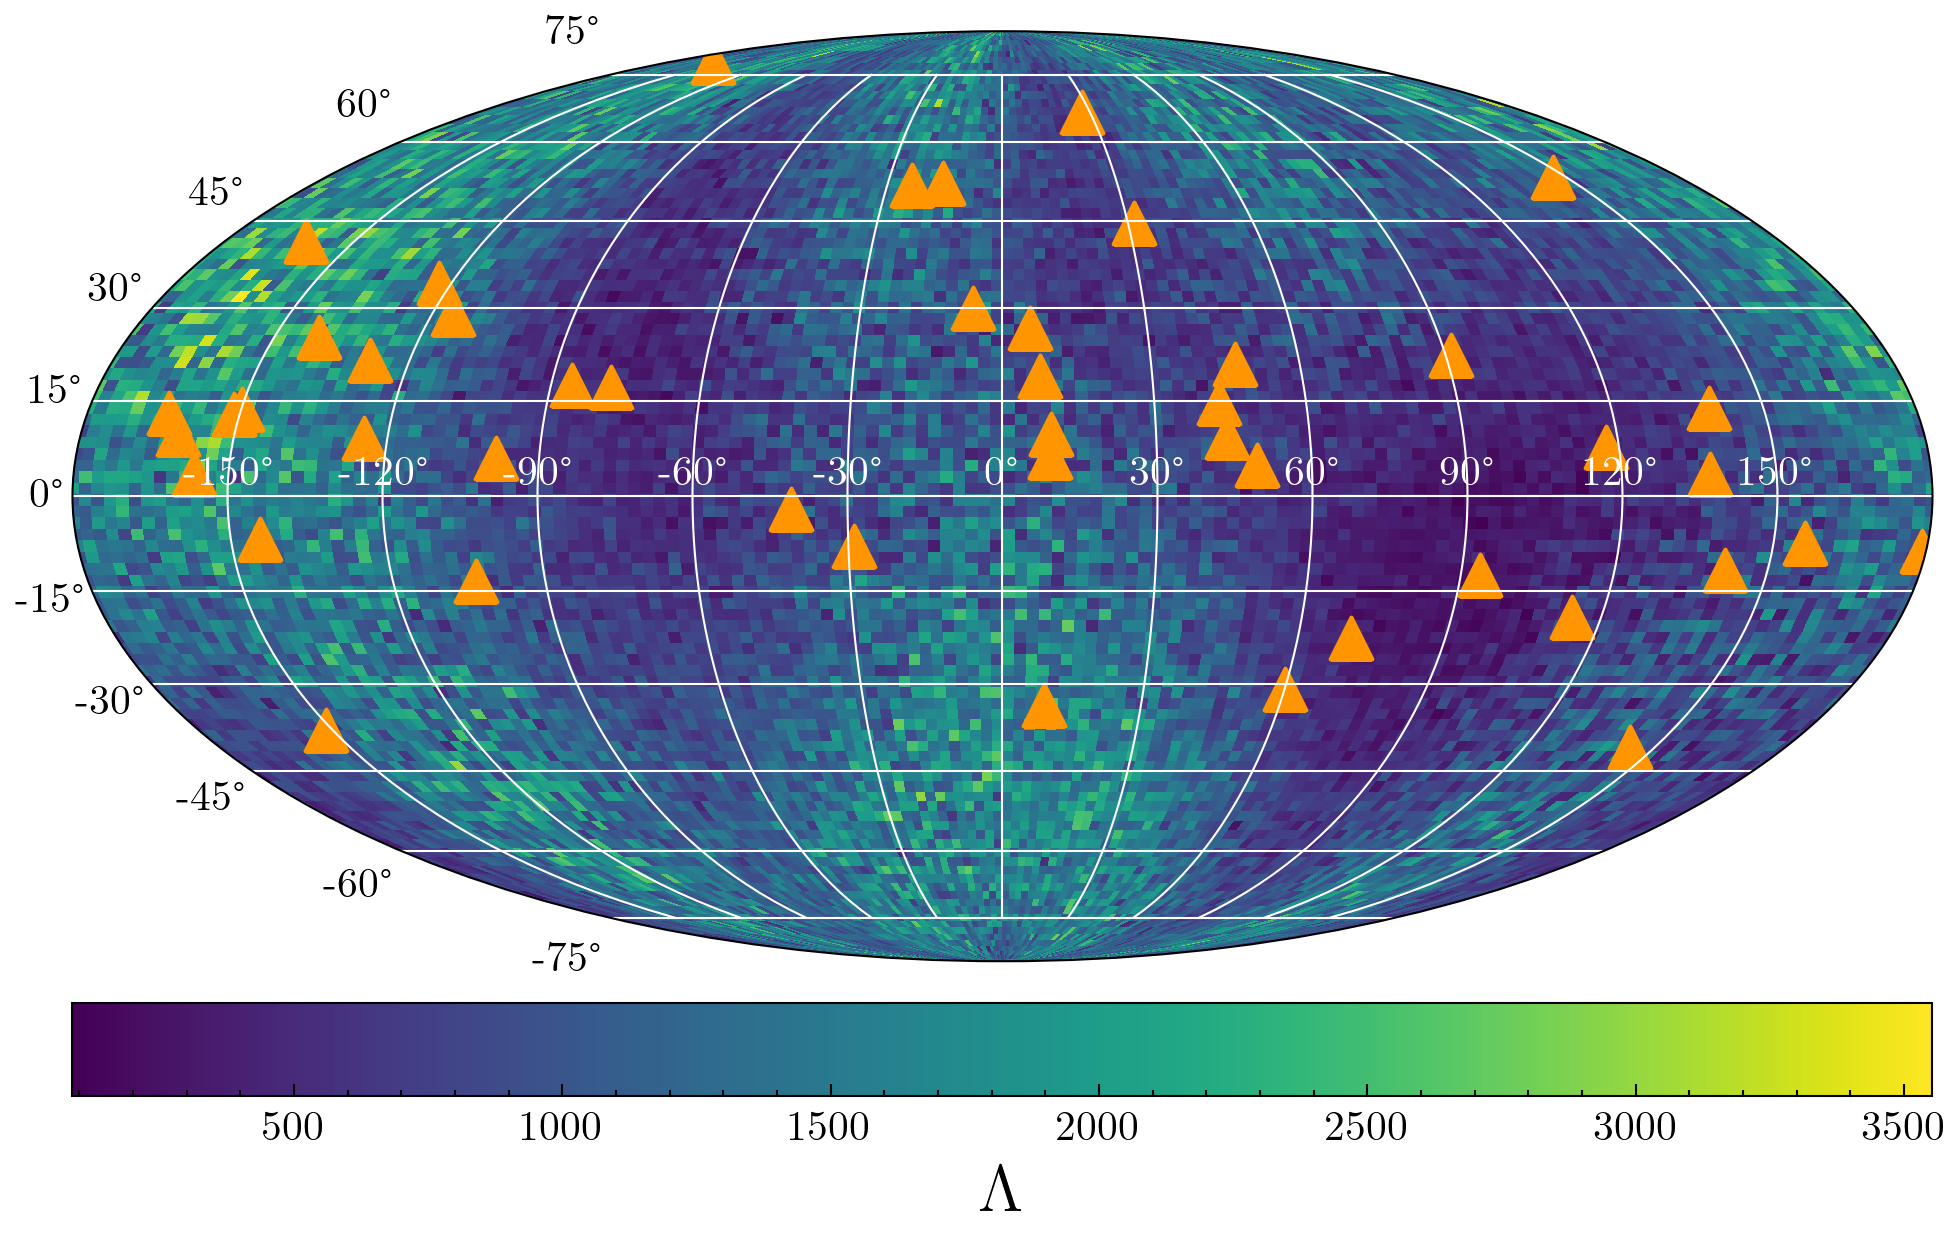
\includegraphics[width=0.8\textwidth]{images/snr_mollewide}
	\caption{\textcolor{red}{TK: Just a placeholder. Likelihood ratio for a given $h$. Maybe more interesting, but more expensive, to get minimum detectable h?}}
	\label{fig:mollewide}
\end{figure*}




%
%
%
%\begin{figure}
%	%\centering % Not needed
%	\begin{subfigure}[b]{1\columnwidth}
%		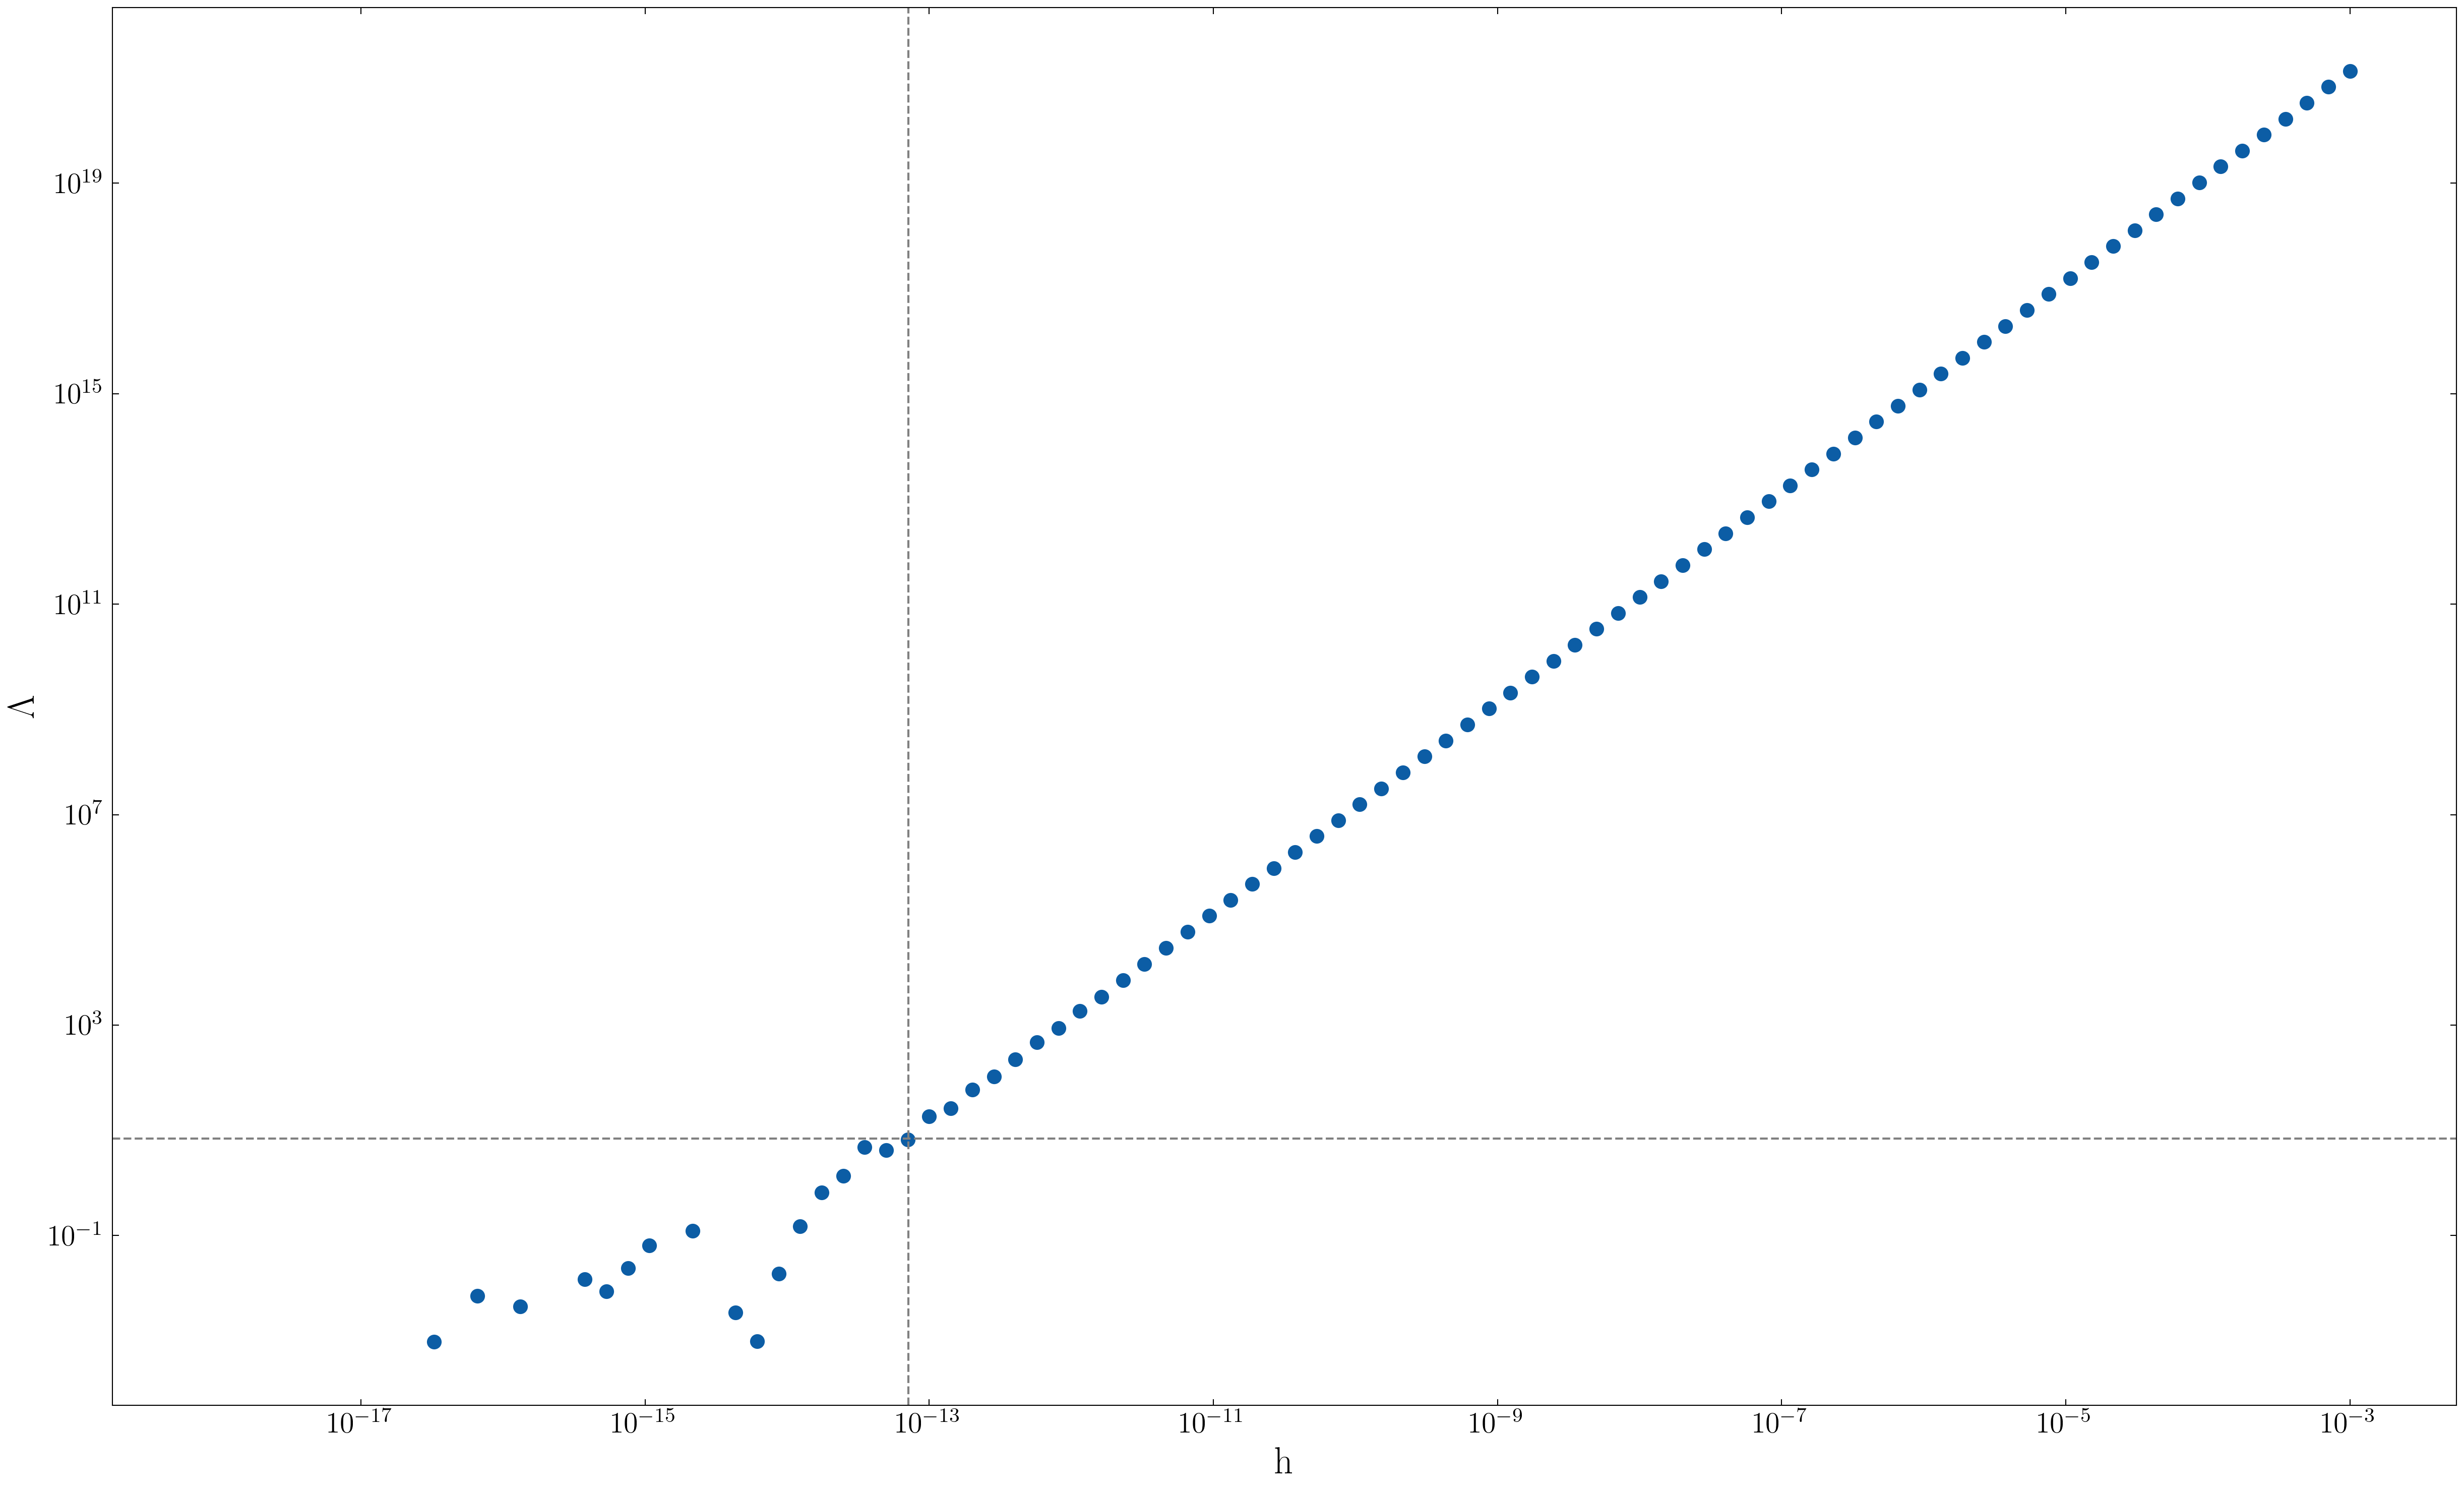
\includegraphics[width=\textwidth]{images/snr_canonical}
%		\caption{}
%		\label{fig:6MB_BFS}
%	\end{subfigure}
%	\\
%	\begin{subfigure}[b]{1\columnwidth}
%		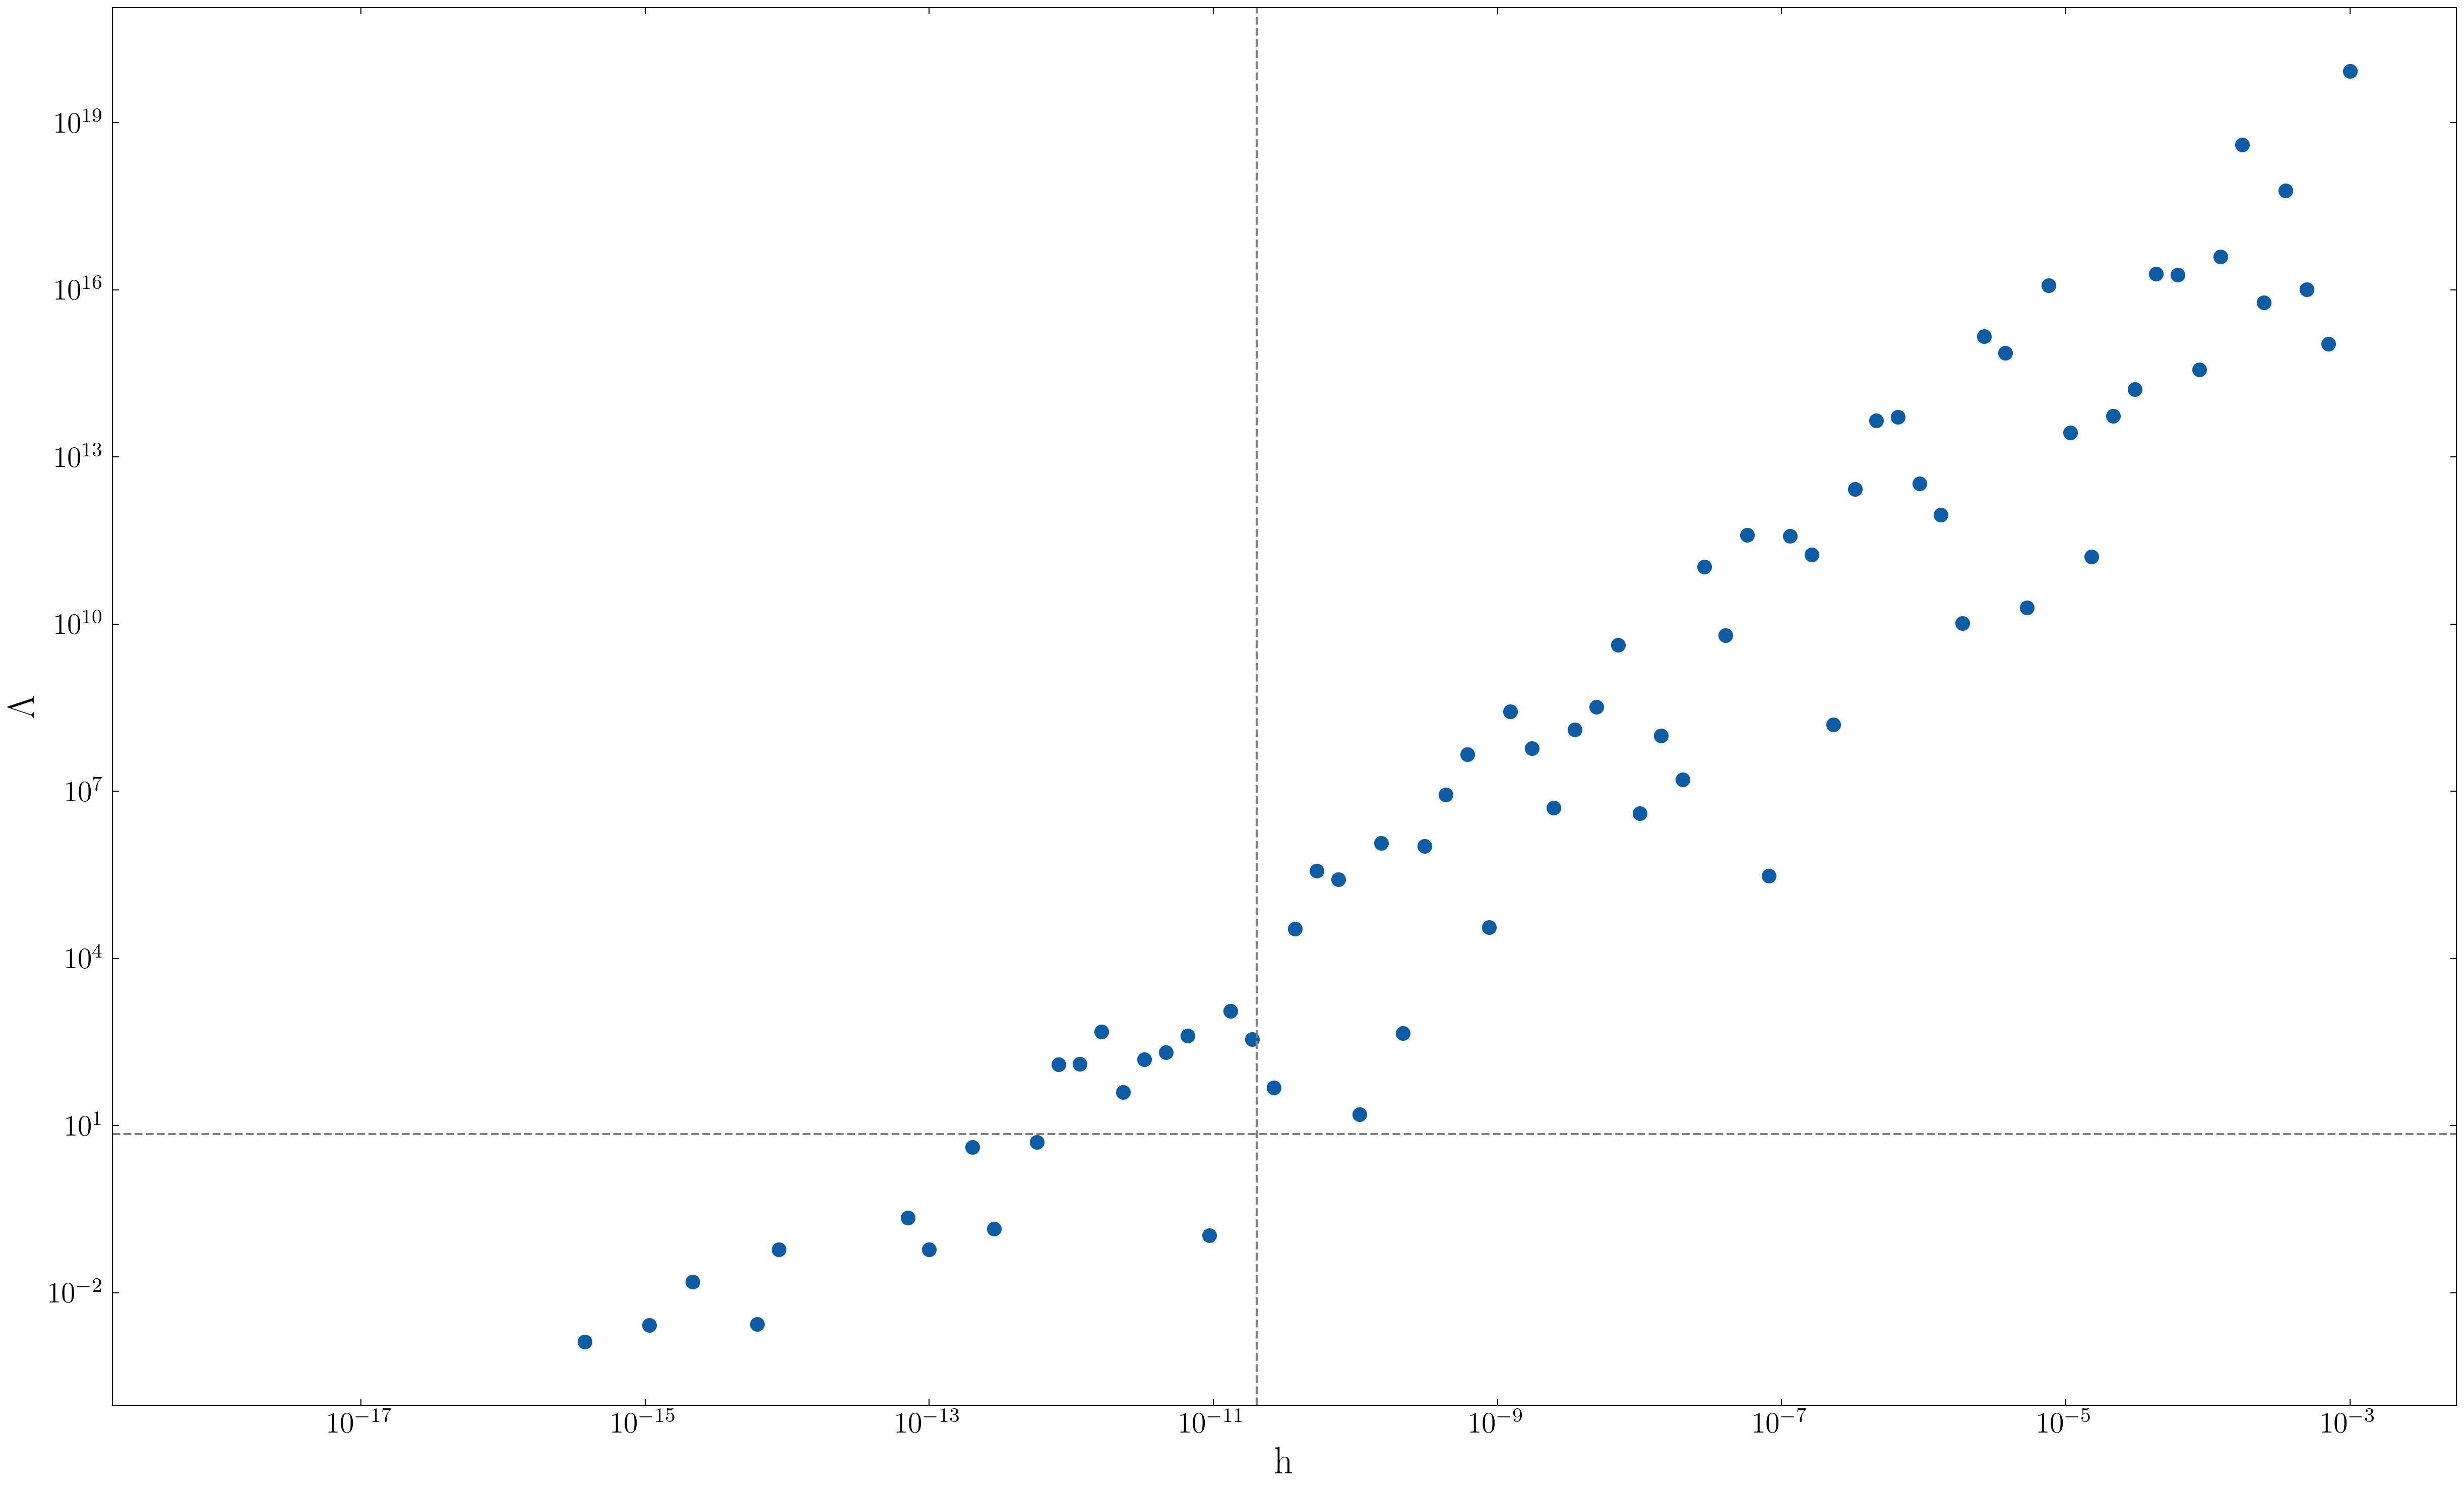
\includegraphics[width=\textwidth]{images/snr_canonical_1psr}
%		\caption{}
%		\label{fig:25MB_bfs}
%	\end{subfigure}
%	\caption{}
%	\label{fig:snr_detection}
%\end{figure}








\section{Discussion}

Points to discuss:

\begin{itemize}
	\item Non constant time sampling? Different pulsars sampled at different times...
\end{itemize}

\section{Conclusion}

Questions 

\begin{itemize}
	\item PTAs like MSPs for small timing noise. Can we get away with large timing noise, and use more pulsars? Some pulsars are more useful than others, e.g. arXiv 2211.03201
	\item Can we also estimate radiometer noise? Is this useful?
\end{itemize}





\appendix

\section{Kalman recursion equations} \label{sec:kalman}










The linear Kalman filter operates on temporally discrete measurements which are related to unobservable system states via a linear transformation
\begin{equation}
	\bar{z} = \bar{H} \bar{x} + \bar{v}
\end{equation}
where $\bar{H}$ is the measurement matrix and $\bar{v}$ is a Gaussian measurement noise. The underlying states evolve according to are the state-space dynamical equation 
\begin{equation}
	\dot{\bar{x}} = \bar{F} \bar{x} + \bar{G}\bar{u} + \bar{w}
\end{equation}
for the system dynamics matrix,$\bar{F}$,  control model $G$, control vector $\bar{u}$, and $w$ a stochastic zero-mean process. By comparison with the preceding equations, Eqs. 	\ref{eq:state1} - 	\ref{eq:state2}, it is immediately obvious how our state space model maps onto the Kalman filter structure. Specifically, our states are just the $N$ intrinsic pulsar frequencies $\bar{x} = (f_1,f_2,...f_N)$ whilst our measurements are the $N$ measured pulse frequencies $\bar{z} = (f^{(M)}_1,f^{(M)}_2,...f^{(M)}_N)$. If we specialize to the case of constant time sampling between our observations, $\Delta t$, then for our formulation the components that make up the Kalman filter are as follows: 
\begin{equation}
	F_i = F_{i+1} = e^{-\gamma \Delta t}
	\label{eq:fmatrix}
\end{equation}
\begin{align}
	T_i &= \int_{t_i}^{t_{i+1}}  e^{A (t_{i+1} - t')} N(t') dt' \\
	& = f_{\rm EM}(0) + \dot{f}_{\rm EM}(0)  (\Delta t + t_i) - e^{-\gamma \Delta t} (f_{\rm EM}(0) + \dot{f}_{\rm EM}(0)t_i)
\end{align}
\begin{equation}
	H_i = 1 -A(\theta_{\rm GW}) \cos(-\Omega t_i (1 + n\cdot q ) + \Phi_0)
\end{equation}
where the $i$ subscript labels the value at the $i$-th timestep, and $A$ is a constant that is given by  Eq. \ref{eq:state2}. \newline 


\noindent The Kalman filter includes the effect of process noise $\bar{w}$ and the measurement noise $\bar{v}$ via the definition of a process noise matrix $Q = E[w w^T]$ and a measurement noise matrix $R = E[v v^T]$, which have the discrete form,
\begin{equation}
	Q_i  \delta_{ij}= \langle \eta_i \eta_j^T \rangle = \frac{- \sigma^2}{2 \gamma} \left( e^{-2 \gamma \Delta t} -1\right)
\end{equation}
\begin{equation}
	R_i = R_{i+1} = \Sigma^2
	\label{eq:rmatix}
\end{equation}
The above equations, Eqs. \ref{eq:fmatrix} - 	\ref{eq:rmatix}, apply to an operation on a single state. The extension to $N$ states is straightforward, since one just needs to construct a diagonal matrix for each of the Kalman components where each non-zero element corresponds to a separate pulsar frequency. 





In Section \ref{sec:statespace} we present a discretised version of the model of Section \ref{sec:model} which maps onto the discretely sampled observable $f(\tau)|_{\rm Earth}$. 





In order to make contact with discretely sampled data it is importnat to temporally discretise the model of Section \ref{sec:model}


We can express the intrinsic frequency evolution, Eq. \ref{eq:frequency_evolution_expanded}, in a alternative form as,
\textcolor{red}{TK all this needs updating}
\begin{equation}
	df = \gamma  f dt + N(t) dt + \sigma dB(t)
	\label{eq:state1}
\end{equation}
where $\mathcal{A} = -\gamma$, $N(t) = \gamma(f_{\rm EM}(0) + \dot{f}_{\rm EM}(0) t) +\dot{f}_{\rm EM}(0)$ and $dB(t)$ denotes increments of Brownian motion (Wiener process). This equation is easily identified as an Ornstein-Uhlenbeck process which has a general solution given by \citep{gardiner2009stochastic},
\begin{equation}
	f(t) = e^{\mathcal{A}t}f(0) + \int_0^t e^{\mathcal{A}(t-t')} N(t') dt' + \int_0^t e^{\mathcal{A}(t-t')} \sigma dB(t')
\end{equation} 
If we move from a solution in continuous time, $t$, to discrete time, \textcolor{red}{TK: AM reccomends deligint tabe sy,bol} $\bar{t} = (t_1, t_2, ...,t_K)$, then
\begin{equation}
	f(t_{i+1}) = F f(t_i) + T_i + \eta_i
\end{equation}
where
\begin{equation}
	F_i = e^{\mathcal{A} (t_{i+1} - t_i)}
\end{equation}
\begin{equation}
	T_i = \int_{t_i}^{t_{i+1}}  e^{\mathcal{A} (t_{i+1} - t')} N(t') \, dt'
\end{equation}
\begin{equation}
	\eta_i = \int_{t_i}^{t_{i+1}}  e^{\mathcal{A} (t_{i+1} - t')} \sigma \, dt'
\end{equation}

if we specialise to the case of constatn time sampling 






The discrete solution $f(\bar{t})$ to the intrinsic frequency can be related to the discrete measured frequency via Eq. \ref{eq:main_eq} as,
\begin{equation}
	f_M (\bar{t})= f(\bar{t}) g(\bar{\theta},\bar{t}) + N_M
\end{equation}
where $g(\theta,t)$ can be expressed in a trigonometric form as 
\begin{equation}
	X = 1 - \frac{1}{2} \frac{ H_{ij}q^i q^j }{(1 + \bar{n}\cdot \bar{q}) } \left[ \cos(-\Omega \tau +\Phi_0) - \cos(-\Omega \tau +\Phi_0 + \Omega (1 + \bar{n}\cdot \bar{q})  d) \right]
\end{equation} 
whilst $N_M$ is a Gaussian measurement noise that satisfies 
\begin{equation}
	\langle N_M(t) N_M(t') \rangle = \Sigma^2 \delta(t - t')
\end{equation}
for variance $\Sigma^2$. 









\subsection{References}
\label{sec:ref_list}





\bibliographystyle{mnras}
\bibliography{example} % if your bibtex file is called example.bib





%%%%%%%%%%%%%%%%%%%%%%%%%%%%%%%%%%%%%%%%%%%%%%%%%%


% Don't change these lines
\bsp	% typesetting comment
\label{lastpage}
\end{document}

% End of mnras_guide.tex
